\chapter{Negative Polarity Items in Conditional Antecedents}\labch{npi-conditionals}
In this chapter, we examine the interaction between the \textit{even}-based approach to NPI licensing and the two predominant approaches to conditional semantics: the variably-strict approach \parencite{Stalnaker1968,Lewis1973} as well as the (semi-)dynamic strict approach \parencite{Fintel2001,Gillies2007}. We do this to better tease apart the predictions that result from the two approaches to conditionals, to further the debate on which model more accurately reflects speaker use. To accomplish this, we first examine what types of NPIs are licensed in conditionals and which conditions might influence the felicity of their use in conditional antecedents in \refsec{conditional-npi-data}. This is followed by an examination of the interaction between the \textit{even}-based approach and \textcite{Stalnaker1968} and \citepos{Lewis1973} variably-strict semantics in \refsec{conditional-npi-vss}. We then examine the same interaction with \citepos{Fintel2001} (semi-)dynamic strict semantics in \refsec{conditional-npi-sss}. Finally, in \refsec{conditional-npi-conclusion}, we provide an intermediate conclusion for this chapter and its impact on  the debate between a variably-strict conditional semantics and a (semi-)dynamic strict conditional semantics.

\section{Empirical Data on NPIs in Conditionals}\labsec{conditional-npi-data}
The traditional view is that all those NPIs that we have classified as weak in \refsec{npi-taxonomy} \parencite{Ladusaw1980,Wouden1997,Jeong2021,Jeong2022} are licensed in the antecedent of conditionals. We show this in \refex{npi-conditional-good-any}, \refex{npi-conditional-good-ANY}, and \refex{npi-conditional-good-finger}. In addition, the expression \textit{even \MakeUppercase{one}} is also typically licensed in such constructions, as shown in \refex{even-conditional-good-even}.
\pex[nopreamble=true]\phantomsection\label{ex:npi-conditional-good}%
\a\phantomsection If John had read any book, he would've passed the test.\labex{npi-conditional-good-any}
\a\phantomsection If John had read \MakeUppercase{any} book, he would've passed the test.\labex{npi-conditional-good-ANY}
\a\phantomsection If John had lifted a finger during class, he would've passed the test.\labex{npi-conditional-good-finger}
\a\phantomsection If John had read even \MakeUppercase{one} book, he would've passed the test.\labex{even-conditional-good-even}
\xe
However, the felicity of weak NPIs and of the expression \textit{even \MakeUppercase{one}} in conditional antecedents appears to be by no means guaranteed. \textcite[p.~122]{Crnic2014-dogma} argues that the distribution of weak NPIs in conditional antecedents is akin in its context-sensitivity to that of Strawson downward monotone environments such as the restrictor of universal quantification: I.e., emphatic \textit{any} and minimisers display some degree of context-sensitivity, whereas the unfocused weak NPI \textit{any} should not. We show this in \refex{npi-conditional-bad-any}, \refex{npi-conditional-bad-ANY}, and \refex{npi-conditional-bad-finger}. In addition, the expression \textit{even \MakeUppercase{one}} also appears to be unlicensed in such contexts, as shown in \refex{even-conditional-bad-even}.
\pex[nopreamble=true]\phantomsection\label{ex:npi-conditional-bad}%
\a\phantomsection\ljudge{} If John had read any book, he would've worn blue jeans.\labex{npi-conditional-bad-any}
\a\phantomsection\ljudge{\#} If John had read \MakeUppercase{any} book, he would've worn blue jeans.\labex{npi-conditional-bad-ANY}
\a\phantomsection\ljudge{\#} If John had lifted a finger in class, he would've worn blue jeans.\labex{npi-conditional-bad-finger}
\a\phantomsection\ljudge{\#} If John had read even \MakeUppercase{one} book, he would've worn blue jeans.\labex{even-conditional-bad-even}
\xe
Here, the use of NPIs in \refex{npi-conditional-bad-ANY} and \refex{npi-conditional-bad-finger} is clearly unlicensed in a context where the antecedent and the consequent of the conditional have no apparent correlation. As such, it would appear that some NPIs---namely emphatic \textit{any} and minimisers---are context-sensitive insofar as that they require a clear link between their use in the antecedent and the intended causative correlation towards their consequent.

However, the case of unfocused NPIs in conditional antecedents is not as clear: While \textcite{Crnic2014-dogma} implicitly claimed that they should be felicitous regardless of any causation between antecedent and consequent\footnote{We say that \textcite{Crnic2014-dogma} only claimed this implicitly as he did not provide any concrete conditional examples nor did he specifically say that unfocused weak NPIs should be felicitous in conditional antecedents. He merely stated that the distribution and context-sensitivity of weak NPIs in conditionals appears to be equal to their distribution in the restrictor of universal quantifiers \parencite[p.~122--124]{Crnic2014-dogma}. This should entail that we should be able to use them felicitously in \refex{npi-conditional-bad-any}.}, our preliminary and limited feedback from native speakers appears mixed: Some find \refex{npi-conditional-bad-any} to only be marginally better than \refex{npi-conditional-bad-ANY}, others find them equally infelicitous, and only some few find \refex{npi-conditional-bad-any} to be substantially better than \refex{npi-conditional-bad-ANY}. As such, our actually observed felicity distribution of weak NPIs and \textit{even \MakeUppercase{one}} is actually closer to the one shown in \refex{npi-conditional-bad-actual}---where we signify this mostly negative mixture of judgements with the symbol \%---rather than the one shown in \refex{npi-conditional-bad}.
\pex[nopreamble=true]\phantomsection\label{ex:npi-conditional-bad-actual}%
\a\phantomsection\ljudge{\%} If John had read any book, he would've worn blue jeans.\labex{npi-conditional-bad-any-actual}
\a\phantomsection\ljudge{\#} If John had read \MakeUppercase{any} book, he would've worn blue jeans.\labex{npi-conditional-bad-ANY-actual}
\a\phantomsection\ljudge{\#} If John had lifted a finger in class, he would've worn blue jeans.\labex{npi-conditional-bad-finger-actual}
\a\phantomsection\ljudge{\#} If John had read even \MakeUppercase{one} book, he would've worn blue jeans.\labex{even-conditional-bad-even-actual}
\xe

We do not know, however, if \textcite{Crnic2014-dogma} had such conditional sentences in mind when he made this claim. As such, we turn to the closest possible conditional analogue of the universally quantifying sentences in \refex{even-every-bad}, repeated below as \refex{npi-every-bad-condch}:
\pex[nopreamble=true]\phantomsection\label{ex:npi-every-bad-condch}%
\a\phantomsection Every student in my class who read any book wore blue jeans.
\a\phantomsection\ljudge{\#} Every student in my class who read \MakeUppercase{any} book wore blue jeans.
\a\phantomsection\ljudge{\#} Every student in my class who lifted a finger in class wore blue jeans.
\a\phantomsection\ljudge{\#} Every student in my class who read even \MakeUppercase{one} book wore blue jeans.
\xe
Here, \citepos{Crnic2014-dogma} claimed empirical distribution for conditional analogues of \refex{npi-every-bad-condch} would have been \refex{npi-every-bad-analogue} for non-counterfactuals and \refex{npi-every-bad-analogue2} for counterfactuals, where the unfocused weak NPI yields felicitous conditional sentences but the focused weak NPIs do not.
\pex[nopreamble=true]\phantomsection\label{ex:npi-every-bad-analogue}%
\a\phantomsection\ljudge{} If a student in my class read any book, they wore blue jeans.
\a\phantomsection\ljudge{\#} If a student in my class read \MakeUppercase{any} book, they wore blue jeans.
\a\phantomsection\ljudge{\#} If a student in my class lifted a finger in class, they wore blue jeans.
\a\phantomsection\ljudge{\#} If a student in my class read even \MakeUppercase{one} book, they wore blue jeans.
\xe
\pex[nopreamble=true]\phantomsection\label{ex:npi-every-bad-analogue2}%
\a\phantomsection\ljudge{} If a student in my class had read any book, they would've worn blue jeans.
\a\phantomsection\ljudge{\#} \resizebox{374pt}{!}{If a student in my class had read \MakeUppercase{any} book, they would've worn blue jeans.}
\a\phantomsection\ljudge{\#} If a student in my class had lifted a finger in class, they would've worn blue jeans.
\a\phantomsection\ljudge{\#} If a student in my class had read even \MakeUppercase{one} book, they would've wore blue jeans.
\xe
Instead of this expected distribution, our preliminary feedback for these sentences would suggest an empirical distribution such that the unfocused weak NPI conditionals are again either infelicitous or, at least, degraded (though most judged them to be not as bad as focused weak NPIs in the same context), as shown in \refex{npi-every-bad-analogue3} and \refex{npi-every-bad-analogue4}.
\pex[nopreamble=true]\phantomsection\label{ex:npi-every-bad-analogue3}%
\a\phantomsection\ljudge{\%} If a student in my class read any book, they wore blue jeans.
\a\phantomsection\ljudge{\#} If a student in my class read \MakeUppercase{any} book, they wore blue jeans.
\a\phantomsection\ljudge{\#} If a student in my class lifted a finger in class, they wore blue jeans.
\a\phantomsection\ljudge{\#} If a student in my class read even \MakeUppercase{one} book, they wore blue jeans.
\xe
\pex[nopreamble=true]\phantomsection\label{ex:npi-every-bad-analogue4}%
\a\phantomsection\ljudge{\%} If a student in my class had read any book, they would've worn blue jeans.
\a\phantomsection\ljudge{\#} \resizebox{374pt}{!}{If a student in my class had read \MakeUppercase{any} book, they would've worn blue jeans.}
\a\phantomsection\ljudge{\#} If a student in my class had lifted a finger in class, they would've worn blue jeans.
\a\phantomsection\ljudge{\#} If a student in my class had read even \MakeUppercase{one} book, they would've wore blue jeans.
\xe

It is unclear whether the perceived infelicity of unfocused weak NPIs and of the expression \textit{even \MakeUppercase{one}} in conditional antecedents that have no causative correlation to their consequents is a product of the respective expression itself or of a more general phenomenon pertaining to conditionals: Namely that we generally expect conditional antecedents and consequents to bear a causative correlation \parencite[see, among many others,][]{Douven2008,Schulz2011,Spohn2013,vanRooij2022}.\footnote{Note that these citations treat different kinds of conditionals.\textcite{Schulz2011}, for example, makes this point with regards to counterfactual conditionals only. The remaining citations either make the point for non-counterfactual as well as counterfactual conditionals or only for the former ones.} Consider the counterfactual and non-counterfactual conditional sentences in \refex{bluejeansconditionals}.
\pex\phantomsection\label{ex:bluejeansconditionals}%
\textit{Yesterday, John was wearing blue jeans all day long.}
\a\phantomsection\ljudge{\%} If John read a book yesterday, he was wearing blue jeans.
\a\phantomsection\ljudge{\%} If John had read a book yesterday, he would've been wearing blue jeans.
\xe
These sentences do not contain any NPIs, yet we have also received mixed responses with regards to whether or not they are felicitous or infelicitous, though most of the feedback agreed that they would deem the sentences themselves to be true, given the context. While some have indicated that they found the sentences in \refex{bluejeansconditionals} to be marginally better than their equivalent containing an unfocused weak NPI, others have not indicated this. 

As such, we would argue that we do not have enough data at the moment to definitively settle the issue of whether or not the introduction of weak NPIs in the antecedent of such conditionals further degrades their acceptability. However, there are three differentiable possibilities, of which the first two are closely related: 

First, \textcite{Crnic2014-dogma} is entirely correct, and the causal link between antecedent and consequent is only of any importance to conditionals containing a focused weak NPI. This can be tentatively ruled out, given our preliminary feedback and preexisting literature concerning the nature of conditionals \parencite{Douven2008,Schulz2011,Spohn2013,vanRooij2022}. This particular hypothetical empirical distribution is shown in \reftab{even-taxonomy-crnic}.
\begin{table}[!htb]
\caption{Felicity distribution for weak NPIs and the expression \textit{even \MakeUppercase{one}}. For question contexts, \textit{Strong}, \textit{Weak}, and \textit{$\emptyset$} refer to the negative strength of the context (i.e., how many alternative questions are negatively settled) and the checkmarks indicate whether the use of the NPI is licensed in these contexts. Sorted by average acceptability.}
\resizebox{\textwidth}{!}{
    \begin{tabular}{lccccc>{\columncolor[gray]{0.85}}c>{\columncolor[gray]{0.85}}cccccc}\toprule
            \multirow{2}{*}{Construction}     & Negative & Negative & \multicolumn{3}{c}{\multirow{2}{*}{Question}} & \multicolumn{2}{>{\columncolor[gray]{0.85}}c}{Conditional} & \multicolumn{2}{c}{Universal} & \multicolumn{2}{c}{\multirow{2}{*}{Exactly $n$}} & Simple\\
             & Particle & Quantifier &  &  & & \multicolumn{2}{>{\columncolor[gray]{0.85}}c}{Antecedent} & \multicolumn{2}{c}{Quantifier} & & & Affirmative\\\midrule
            Context & & & Strong & Weak & $\emptyset$ & Link & No Link & Link & No Link & Low & High\\\midrule
            Unfocused NPI                 & \checkmark & \checkmark & \checkmark & \checkmark &\checkmark & \checkmark & \checkmark & \checkmark & \checkmark & \checkmark & \# & \#\\
            Contingently Focused NPI & \checkmark & \checkmark & \checkmark & \checkmark & \# & \checkmark & \# & \checkmark & \# & \checkmark & \# & \#\\
            Inherently Focused NPI       & \checkmark & \checkmark & \checkmark & \# & \# & \checkmark & \# & \checkmark & \# & \checkmark & \# & \#\\
            Even \MakeUppercase{one}       & \checkmark & \checkmark & \checkmark & \# & \# & \checkmark & \# & \checkmark & \# & \checkmark & \# & \#\\
          \bottomrule
    \end{tabular}
}\labtab{even-taxonomy-crnic}
\end{table}

Second, \textcite{Crnic2014-dogma} is correct in assuming that focused weak NPIs exhibit a degree of context-sensitivity in antecedents that unfocused weak NPIs do not. However, the general need of conditionals to have an appropriate correlation between antecedent and consequent masks this fact---to an extent---by degrading conditionals without an appropriate causal link, but a contrast between focused and unfocused is expected and can still be detected. This possible empirical distribution is shown in \reftab{even-taxonomy-ch2}, where ?\# signifies a degraded sentence that is contrastively more acceptable than a sentence marked with \#.
\begin{table}[!htb]
\input{content/tables/even-taxonomy-crnic}\labtab{even-taxonomy-ch2}
\end{table}

Third, the general need of conditionals to have a sensible causal relation between antecedent and consequent renders such constructions infelicitous to such a degree that no contrast is be detectable, regardless of any presuppositions carried by \textit{even \MakeUppercase{one}} or by weak NPIs. This particular possible empirical distribution is shown in \reftab{even-taxonomy-nocrnic}, where \textit{N.A.} is the abbreviation for \textit{Not Applicable}.
\begin{table}[!htb]
\input{content/tables/even-taxonomy-nocrnic}\labtab{even-taxonomy-nocrnic}
\end{table}

Generally speaking, the first two possibilities that (more or less) correspond to \citepos{Crnic2014-dogma} expected distribution and can be characterised as requiring there to be some kind of contrast between unfocused and focused NPIs, whereas the third possibility expects that there is no possibility of detecting a contrast between these types of NPIs.

Of these possibilities, the one that best fits our preliminary feedback is the second one, shown in \reftab{even-taxonomy-ch2}. We assume this particular possibility to be the case for the remainder of this chapter. However, we return to consider the other possible felicity distributions in \refsec{conditional-npi-conclusion} and see how compatible they are to each model.

\section{Variably-Strict Semantics}\labsec{conditional-npi-vss}
\textcite{Stalnaker1968} and \textcite{Lewis1973} assume that any conditional \enquote{If $\phi$, $\psi$} is true iff all the closest $\phi$-worlds are also $\psi$-worlds, as defined in \refdef{variablystrict-intro} and \refdef{variablystrictformal-intro}, as repeated below in \refdef{variablystrict-npisection2} and \refdef{variablystrictformal-npisection}, where the accessibility function $f_\leqslant(p,w)$ returns the set of the $p$-worlds that are closest to the evaluation world $w$.
\ex\phantomsection\labdef{variablystrict-npisection2}For all contexts $c$, \enquote{If $\phi$, $\psi$} is true at $w$ in $c$ iff all the closest $\phi$-worlds to $w$ are $\psi$-worlds, where closeness is determined by similarity.%
\xe
\ex\phantomsection\labdef{variablystrictformal-npisection}$\intension{If $\phi$, $\psi$}=[\lambda w_s.\forall v:v\in f_\leqslant([\lambda w'_s.\phi(w')],w)[\psi(v)]]$\xe
Given this basic semantics, the generalised variant of the conditionals in \refex{even-conditional-good-even} and \refex{even-conditional-bad-even}, provided in \refex{vs-neutral-conditional-sentence} below, would have the LF in \refex{vs-neutral-conditional-lf}. Said LF would, in turn, yield the assertive meaning in \refex{vs-neutral-conditional-assertion}, the set of alternatives in \refex{vs-neutral-conditional-alternatives}, as well as the probability-based scalar presupposition in \refex{vs-neutral-conditional-even}.
\pex[nopreamble=true]\phantomsection\label{ex:vs-neutral-conditional}%
\a\phantomsection If John had read even \MakeUppercase{one} book, IP.\labex{vs-neutral-conditional-sentence}
\a[]\phantomsection [even\textsubscript{C} [If John had read one\textsubscript{F} book IP]]\labex{vs-neutral-conditional-lf}
\a\phantomsection $\intension[g,c]{If John had read one\textsubscript{F} book, IP}=$\\$[\lambda w_s.\forall v:v\in f_\leqslant([\lambda w'_s.\exists{x}[\predicate{read}(j,x,w')\land\predicate{book}(x,w')]],w)[\predicate{ip}(v)]]$\labex{vs-neutral-conditional-assertion}
\a\phantomsection $\intension[f,g,c]{If John had read one\textsubscript{F} book, IP}=$\\$\{[\lambda w_s.\forall v:v\in f_\leqslant([\lambda w'_s.\exists_n{x}[\predicate{read}(j,x,w')\land\predicate{book}(x,w')]],w)[\predicate{ip}(v)]]$\\\emptyfill$~|~n\in\mathbb{N}\geqslant1\}$\labex{vs-neutral-conditional-alternatives}
\xe

\ex\phantomsection
$\intension[g,c]{even\textsubscript{C}}(\intension[g,c]{If John had read one\textsubscript{F} book, IP})(w)$\\ is defined in $w$ only if for all $n\in\mathbb{N}>1$:\\
$\forall v:v\in f_\leqslant([\lambda w'_s.\exists_1{x}[\predicate{read}(j,x,w')\land\predicate{book}(x,w')]],w)[\predicate{ip}(v)]~\lprob_c$\\\emptyfill$\forall v:v\in f_\leqslant([\lambda w'_s.\exists_n{x}[\predicate{read}(j,x,w')\land\predicate{book}(x,w')]],w)[\predicate{ip}(v)]$\labex{vs-neutral-conditional-even}
\xe
To evaluate whether or not the probability relation holds true, we must consider the relation between the alternatives. In the variably-strict analysis of conditionals, $\intension[g,c]{If John had read one book, IP}$ does not entail $\intension[g,c]{If John had read n books, IP}$ for $n>1$, as the world selection function exclusively selects worlds that fulfil its respective antecedent and are maximally close to the evaluation world. In this specific case, where the different antecedents relate to how many books John has read, each counterfactually read book decreases the respective world similarity to the actual world by one, resulting in the disjoint domains shown in \reffig{evenone-stalnaker}. 
\begin{figure}[!htb]
    \centering
    \resizebox{\linewidth}{!}{    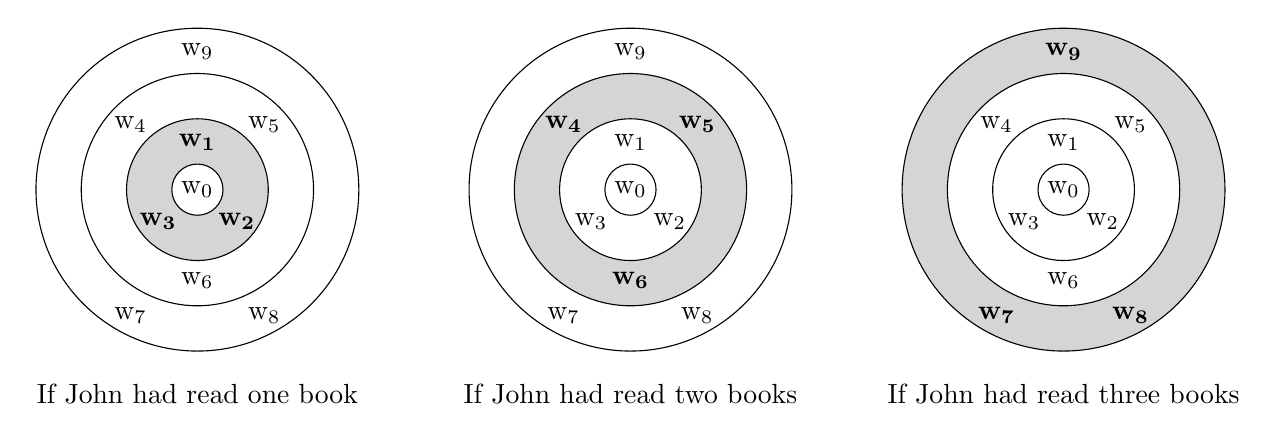
\begin{tikzpicture}
	\coordinate (O) at (0,0);
	\draw[fill=white] (O) circle (2.05);
	\draw[fill=white] (O) circle (1.475);
	\draw[fill=gray!33] (O) circle (0.9);
	\draw[fill=white] (O) circle (0.325)node {w\textsubscript{0}};

	\node at (0,0.6) {\textbf{w\textsubscript{1}}};
	\node at (0.5,-0.4) {\textbf{w\textsubscript{2}}};
	\node at (-0.5,-0.4) {\textbf{w\textsubscript{3}}};
	
	\node at (-0.85,0.825) {w\textsubscript{4}};
	\node at (0.85,0.825) {w\textsubscript{5}};
	\node at (0,-1.15) {w\textsubscript{6}};
	
	\node at (-0.85,-1.6) {w\textsubscript{7}};
	\node at (0.85,-1.6) {w\textsubscript{8}};
	\node at (0,1.75) {w\textsubscript{9}};
	
	\node at (0,-2.6) {If John had read one book};
	
	
	\begin{scope}[xshift=5.5cm]
		\coordinate (O) at (0,0);
    \draw[fill=white] (O) circle (2.05);
	\draw[fill=gray!33] (O) circle (1.475);
	\draw[fill=white] (O) circle (0.9);
	\draw[fill=white] (O) circle (0.325)node {w\textsubscript{0}};

	\node at (0,0.6) {w\textsubscript{1}};
	\node at (0.5,-0.4) {w\textsubscript{2}};
	\node at (-0.5,-0.4) {w\textsubscript{3}};
	
	\node at (-0.85,0.825) {\textbf{w\textsubscript{4}}};
	\node at (0.85,0.825) {\textbf{w\textsubscript{5}}};
	\node at (0,-1.15) {\textbf{w\textsubscript{6}}};
	
	\node at (-0.85,-1.6) {w\textsubscript{7}};
	\node at (0.85,-1.6) {w\textsubscript{8}};
	\node at (0,1.75) {w\textsubscript{9}};
	
	\node at (0,-2.6) {If John had read two books};
	
	\begin{scope}[xshift=5.5cm]
		\coordinate (O) at (0,0);
    \draw[fill=gray!33] (O) circle (2.05);
	\draw[fill=white] (O) circle (1.475);
	\draw[fill=white] (O) circle (0.9);
	\draw[fill=white] (O) circle (0.325)node {w\textsubscript{0}};

	\node at (0,0.6) {w\textsubscript{1}};
	\node at (0.5,-0.4) {w\textsubscript{2}};
	\node at (-0.5,-0.4) {w\textsubscript{3}};
	
	\node at (-0.85,0.825) {w\textsubscript{4}};
	\node at (0.85,0.825) {w\textsubscript{5}};
	\node at (0,-1.15) {w\textsubscript{6}};
	
	\node at (-0.85,-1.6) {\textbf{w\textsubscript{7}}};
	\node at (0.85,-1.6) {\textbf{w\textsubscript{8}}};
	\node at (0,1.75) {\textbf{w\textsubscript{9}}};
	
	\node at (0,-2.6) {If John had read three books};
	\end{scope}
	\end{scope}
\end{tikzpicture}}
    \caption{Domains of quantification for \enquote{If John had read \MakeUppercase{one} book, IP} and some of its alternatives according to \textcite{Stalnaker1968} and \citepos{Lewis1973} variably-strict conditional analyses. For all $w_n$-worlds: If $1\leqslant n\leqslant 3$, then John read read one book in $w_n$, and if $4\leqslant n\leqslant 6$, then John read two books $w_n$. If $n\geqslant 7$, then John read at least three books.}
    \labfig{evenone-stalnaker}
\end{figure}
Due to this, the variably-strict semantics is non-monotone by nature. As such, since \citepos{Kolmogorov1933} third axiom of probability does not determine the hierarchy of probabilities for the propositions contained by the set of alternatives, whether or not the probability of $\intension[g,c]{If John had read one book, IP}$ is less than the probability of $\intension[g,c]{If John had read n books, IP}$ for all $n>1$ depends entirely upon the context (i.e., speaker assumptions). In this regard, the non-monotone variably-strict semantics of \textcite{Stalnaker1968} and \textcite{Lewis1973} behaves alike with the other non-monotone environments, as shown in \refsec{even-nm}. In order to ensure that the original prejacent is the least likely member of its set, we would generally have to assume that the probability of the IP increases with the total number of books read (or, at the very least, that there is a one time increase in the IP's probability between having read one book and having read more than one book). As such, \textit{even \MakeUppercase{one}} in conditionals requires some causative correlation between the antecedent and the consequent of the conditional. This is prediction is perfectly in line with the felicity distribution of \textit{even \MakeUppercase{one}} that was shown in \refsec{even-distribution}. For the sentence in \refex{even-conditional-good-even}, the scalar presupposition would be as shown in \refex{vs-good-conditional-even}.
\ex\phantomsection
\resizebox{395pt}{!}{$\intension[g,c]{even\textsubscript{C}}(\intension[g,c]{If John had read one\textsubscript{F} book, he would have passed the test})(w)$}\\ is defined in $w$ only if for all $n\in\mathbb{N}>1$:\\
\resizebox{395pt}{!}{$\forall v:v\in f_\leqslant([\lambda w'_s.\exists_1{x}[\predicate{read}(j,x,w')\land\predicate{book}(x,w')]],w)[\predicate{pass}(j,\iota{y}[\predicate{test}(y,v)],v)]~\lprob_c$}\\
\resizebox{395pt}{!}{$\forall v:v\in f_\leqslant([\lambda w'_s.\exists_n{x}[\predicate{read}(j,x,w')\land\predicate{book}(x,w')]],w)[\predicate{pass}(j,\iota{y}[\predicate{test}(y,v)],v)]$}\labex{vs-good-conditional-even}
\xe
Arguably, this scalar probability presupposition is easily fulfilled or at least accommodated for: There is an obvious link between reading (relevant) books and passing the test. As such, the probability of success should increase with the number of books read, making the probability of success with having read only one book the least likely option in the set of alternatives. As such, this presupposition would be fulfilled, correctly predicting the felicity of \refex{even-conditional-good-even}.

For the sentence in \refex{even-conditional-bad-even}, on the other hand, the scalar presupposition would be as shown in \refex{vs-bad-conditional-even}.
\ex\phantomsection
\resizebox{395pt}{!}{$\intension[g,c]{even\textsubscript{C}}(\intension[g,c]{If John had read one\textsubscript{F} book, he would have worn blue jeans.})(w)$}\\ is defined in $w$ only if for all $n\in\mathbb{N}>1$:\\
\resizebox{395pt}{!}{$\forall v:v\in f_\leqslant([\lambda w'_s.\exists_1{x}[\predicate{read}(j,x,w')\land\predicate{book}(x,w')]],w)[\exists{y}[\predicate{wear}(j,y,v)\land\predicate{jeans}(y,v)]]~\lprob_c$}\\
\resizebox{395pt}{!}{$\forall v:v\in f_\leqslant([\lambda w'_s.\exists_n{x}[\predicate{read}(j,x,w')\land\predicate{book}(x,w')]],w)[\exists{y}[\predicate{wear}(j,y,v)\land\predicate{jeans}(y,v)]$}\labex{vs-bad-conditional-even}
\xe
Here, the scalar probability presupposition posits that the probability of John wearing blue jeans should increase with the number of books read. Barring some bizarre scenarios, this is not typically contextually supported and therefore hard to accommodate for. As such, this presupposition would be unfulfilled, correctly predicting the infelicity of \textit{even \MakeUppercase{one}} in \refex{even-conditional-bad-even}.

However, the fact that the context-sensitivity of \textit{even \MakeUppercase{one}} is already predicted by the basic framework of the variably-strict semantics poses a problem for the analysis of weak NPIs in the framework of the \textit{even}-based licensing theory of NPIs: If context-sensitivity is already predicted for \textit{even \MakeUppercase{one}} without additional covert operations (such as exhaustification), then all weak NPIs would also be predicted to be equally sensitive to context. However, as stipulated in \refsec{conditional-npi-data} and \reftab{even-taxonomy-ch2}, and as exemplified by \refex{npi-conditional-bad-any-actual} and \refex{npi-conditional-bad-ANY-actual}, repeated below as \refex{npi-conditional-bad-any-actual-repeat} and \refex{npi-conditional-bad-ANY-actual-repeat}, this is not the case: Whilst neither conditional is perfectly acceptable, we take the unfocused weak NPI conditional to be somewhat better, on average, than its focused weak NPI counterpart.
\pex[nopreamble=true]\phantomsection%
\a\phantomsection \ljudge{\%}If John had read any book, he would've worn blue jeans.\labex{npi-conditional-bad-any-actual-repeat}
\a\phantomsection\ljudge{\#} If John had read \MakeUppercase{any} book, he would've worn blue jeans.\labex{npi-conditional-bad-ANY-actual-repeat}
\xe
The fact that the variably-strict framework already predicts the context-sensitivity of \textit{even \MakeUppercase{one}} conditionals without additional covert operations is especially problematic for the numeral-based reading of weak NPIs, as its presupposition is essentially identical to the presupposition of overt \textit{even \MakeUppercase{one}}. However, this issue also affects the domain-based reading of weak NPIs. Consider the generalised variant of the conditional \refex{npi-conditional-bad-any-actual-repeat}, provided in \refex{vs-neutral-conditional-any-sentence}, with the LF in \refex{vs-neutral-conditional-any-lf}, the assertive meaning in \refex{vs-neutral-conditional-any-assertion}, the domain-based set of alternatives in \refex{vs-neutral-conditional-any-alternatives}, as well as the resulting scalar presupposition in \refex{vs-neutral-conditional-any-even}:
\pex[nopreamble=true]\phantomsection\label{ex:vs-neutral-conditional-any}%
\a\phantomsection If John had read any book, IP.\labex{vs-neutral-conditional-any-sentence}
\a[]\phantomsection [even\textsubscript{C} [If John had read any book IP]]\labex{vs-neutral-conditional-any-lf}
\a\phantomsection $\intension[g,c]{If John had read any book, IP}=$\\$[\lambda w_s.\forall v:v\in f_\leqslant([\lambda w'_s.\exists{x\in{D^c}}[\predicate{read}(j,x,w')\land\predicate{book}(x,w')]],w)[\predicate{ip}(v)]]$\labex{vs-neutral-conditional-any-assertion}
\a\phantomsection $\intension[g,c]{If John had read any book, IP}_{\text{\scshape alt}}=$\\$\{[\lambda w_s.\forall v:v\in f_\leqslant([\lambda w'_s.\exists{x\in{D'}}[\predicate{read}(j,x,w')\land\predicate{book}(x,w')]],w)[\predicate{ip}(v)]]$\\\emptyfill$~|~D'\subseteq D^c\}$\labex{vs-neutral-conditional-any-alternatives}
\xe
\ex\phantomsection
$\intension[g,c]{even\textsubscript{C}}(\intension[g,c]{If John had read any book, IP})(w)$\\ is defined in $w$ only if for all $D'\subset D^c$:\\
$\forall v:v\in f_\leqslant([\lambda w'_s.\exists{x\in D^c}[\predicate{read}(j,x,w')\land\predicate{book}(x,w')]],w)[\predicate{ip}(v)]~\lprob_c$\\\emptyfill$\forall v:v\in f_\leqslant([\lambda w'_s.\exists{x\in D'}[\predicate{read}(j,x,w')\land\predicate{book}(x,w')]],w)[\predicate{ip}(v)]$\labex{vs-neutral-conditional-any-even}
\xe
Here, we would presuppose that the probability of IP given the assumed fact that John had read at least one book from the domain $D^c$ is less likely than if we had assumed that John had read at least one book from a subdomain $D'$ s.t. $D'\subset D^c$. This presupposition would be enforced by \citepos{Kolmogorov1933} third axiom of probability if we were to assume that $\intension[g,c]{If John had read some D\textsuperscript{c}-book, IP}$ actually entailed $\intension[g,c]{If John had read some D'-book, IP}$ for all respective subdomains. Intuitively speaking, this may often be the case. Imagine the following scenario: There are three books that John had access to, that he could have read without a problem, and that were the only books relevant to the context. As such, we might assume $D^c=\{b_1,b_2,b_3\}$. In this scenario, the counterfactual world in which he read $b_1$ is equally close to $w_0$ as the counterfactual worlds in which he read $b_2$ or $b_3$ are. Let us refer to these worlds as $w_1$, $w_2$, and $w_3$, respectively. Given this scenario, the original conditional would quantify over the closest worlds in which he had read one book from $D^c$: $w_1$, $w_2$, and $w_3$. The alternative conditionals with the domains $D'\subset D^c$ would then quantify over the same degree of world closeness, excluding only one or two worlds of $D^c$ from their domain of quantification, depending on the specific makeup of $D'$. As such, there would be an actual entailment between the original conditional and its alternatives because they all make claims regarding the same worlds, which would allow \citepos{Kolmogorov1933} third axiom of probability to establish the desired probability-based scalar hierarchy.

However, this entailment only holds true when we assume that all elements of $D^c$ share the same degree of world closeness to $w_0$---which is not necessarily given. Assume the following new scenario: There is only one book that John had access to and that he could have read without a problem. In addition, there were two other books relevant to the context that John did not have ready access to. As such, we would still assume that $D^c=\{b_1,b_2,b_3\}$. Now, however, the world in which he had read $b_1$ is not equal in world closeness to $w_0$ as either the world in which he read $b_2$ or the world in which he read $b_3$. We, again, refer to these worlds as $w_1$, $w_2$, and $w_3$, respectively. Here, $w_1$ only requires a single deviance from $w_0$: that John read $b_1$. The worlds $w_2$ and $w_3$ posit one additional deviance to $w_0$: the counterfactual assumption that John had gained access to these books. As such, the original conditional and most of its alternatives would not quantify over the same degree of world closeness. The original conditional, using $D^c$, as well as any $D'$ s.t $b_1\in D'$, would select for the closest antecedent-worlds, which would be $w_1$. Any conditional using a $D'$ s.t. $b_1\not\in D'$, on the other hand, would select for either $w_2$, $w_3$, or both, but never $w_1$. As such, the original conditional does not make a claim regarding all of the worlds selected for by its alternatives, rendering some of their domains disjoint, thereby ensuring that there is no entailing relation between these alternatives. As such, \citepos{Kolmogorov1933} third axiom of probability would create no overarching hierarchy of probability here, rendering the felicity of the expression mostly up to context, same as with the previous numerical reading of weak NPIs or the overt occurrence of \textit{even \MakeUppercase{one}}.

In addition, the exhaustification of the antecedent by {\scshape exh} would also serve no purpose: In a variably-strict semantics, the conditionals \enquote{If John had read one book, IP} and \enquote{If John had read exactly one book, IP} would quantify over the exact same worlds, given that the former selects for the closest worlds where John had read one book---which are all worlds in which John had read exactly one book, as previously shown in \reffig{evenone-stalnaker}, since the reading of a second book would have decreased world closeness to $w_0$. As such, the variably-strict semantics would predict that there is no difference in probability between such conditionals, rendering the use {\scshape exh} in the antecedent on numbers entirely pointless.\footnote{We consider this to be a separate, somewhat unrelated but important failing of this specific account, as, intuitively speaking, the probability of \enquote{If John had read at least one book, IP} should be able to differ from the probability of \enquote{If John had read exactly one book, IP}. In fact, we would argue that the former is intuitively more often than not higher than the latter for most contexts where there is a linear causative correlation between the antecedent and the consequent of a conditional.} 

In sum, the variably-strict approach of \textcite{Stalnaker1968} and \textcite{Lewis1973} fails to predict the correct distribution of NPI felicity by falsely predicting all weak NPIs to be equally sensitive to context rather than predicting unfocused weak NPIs to be marginally better than their focused counterparts. It does, however, account for the context-sensitivity of \textit{even \MakeUppercase{one}} and focused weak NPIs as a consequence of that. The predicted felicity distribution is summarised in \reftab{even-predictions-vs}.%
\begin{table}[!htb]
\caption{Predicted felicity distribution for weak NPIs and \textit{even \MakeUppercase{one}} in conditionals according to a standard variably-strict semantics.}
    \begin{tabular}{lcccc}\toprule
            \multirow{2}{*}{Construction} & \multicolumn{2}{c}{Conditional}\\
                                        & \multicolumn{2}{c}{Antecedent}\\\midrule
            Context                     & Link          & No Link \\\midrule
            Unfocused NPI               & \checkmark    & \#\\
            Contingently Focused NPI    & \checkmark    & \#\\
            Inherently Focused NPI      & \checkmark    & \#\\
            Even \MakeUppercase{one}    & \checkmark    & \#\\
          \bottomrule
    \end{tabular}
\labtab{even-predictions-vs}
\end{table}

\subsection{Dynamic Variably-Strict Semantics}\labsec{dynamicvss}
So far, we have examined the predictions of a variably-strict semantics within its regular static framework. However, \textcite{vanRooij2006} has previously attempted to derive the felicity of NPIs in a variably-strict semantics by adapting it into a dynamic semantic framework such as the \textit{Dynamic Predicate Logic} (DPL) of \textcite{Groenendijk1991}. We therefore must evaluate whether or not the adoption of a dynamic semantics would improve the predictions of a variably-strict semantics with regards to NPI licensing, which is the aim of this subsection.

\textcite{vanRooij2006} set out to accomplish a couple of objectives: Of these, three are of direct importance to this subsection.

First, he attempted to account for an equivalence that is often perceived to be inherent to the majority of so-called donkey sentences, conditionals with the underlying form \enquote{If $\exists{x}P(x)$, $Q(x)$}, such as the one shown in \refex{donkey}, whilst retaining a variably-strict semantics for conditionals.
\ex\phantomsection
If John had owned a donkey, he would have beaten it.\labex{donkey}
\xe
Namely, the donkey sentence \enquote{If $\exists{x}P(x)$, (would-)$Q(x)$} is typically taken to be logically equivalent to the universally quantifying proposition $\forall{x}[P(x)\rightarrow Q(x)]$: Regardless of which donkey John would have counterfactually owned, it is assumed that he would have beaten it. I.e., assuming the domain of donkeys $D_\text{\scshape donkey}=\{d_1,d_2,d_3\}$, \refex{donkey} is equivalent to the conjunction of all conditionals in \refex{donkey-conjunction}.
\pex[nopreamble=true]\phantomsection\label{ex:donkey-conjunction}%
\a\phantomsection If John had owned $d_1$, he would have beaten $d_1$.
\a\phantomsection If John had owned $d_2$, he would have beaten $d_2$.
\a\phantomsection If John had owned $d_3$, he would have beaten $d_3$.
\xe
This kind of donkey sentence reading is also referred to as the \textit{high reading} of indefinites in donkey sentences \parencite{Walker2015}.

Second, \textcite{vanRooij2006} attempted to account for identifying donkey sentences \parencite[p.~393f]{vanRooij2006}, such as \refex{donkey-id}, and weak counterfactual donkey sentences \parencite[first (non-counterfactual) observation due][]{Schubert1987}, such as \refex{donkey-weak}, where this equivalency does not bear out.
\pex[nopreamble=true]\phantomsection%
\a\phantomsection  If Alex had been married to a girl from his class, it would've been Sue.\\\emptyfill\parencite[adapted from][p.~394]{vanRooij2006}\labex{donkey-id}
\a\phantomsection  If I had had a dime in my pocket, I would've thrown it into the meter.\\\emptyfill\parencites[adapted from][]{Schubert1987}[p.~395]{vanRooij2006}\labex{donkey-weak}
\xe
Here, \refex{donkey-id} obviously does not mean that all girls from his class are Sue, and \refex{donkey-weak} does not mean that the speaker would have thrown all of the dimes in his pocket into the meter: Rather, he would only have thrown one of them into it. This kind of reading is also referred to as the \textit{low reading} of indefinites in donkey sentences \parencite{Walker2015}.

Third, and most importantly, he attempted to account for the presence of NPIs in the antecedent of conditionals whilst retaining the fundamental mechanics of a variably-strict semantics. 

To accomplish his first aim, deriving the equivalence to a universally quantified reading for high reading donkey sentences, he adopted the variably-strict semantics into the DPL framework, where the semantic value of any expression is a set of pairs of assignments (an input pair and and output pair), rather than simply a single set of assignments such as in static semantics, allowing us to define which formulas' assignment changes are temporary or permanent. Using this, \textcite{Groenendijk1991} define existential quantification as in \refex{dynamic-exist}.
\ex\phantomsection
$\llbracket\exists x\phi\rrbracket=\{\langle g,h\rangle~|~\exists k:k[x]g\land\langle k,h\rangle\in\llbracket\phi\rrbracket\}$\labex{dynamic-exist}
\xe
\textcite{vanRooij2006} then redefines the ordering relation, making it a partial order over world-assignment pairs where only world-assignments pairs that share an assignment are ranked with respect to one another, as shown in \refdef{rooij-order}.
\ex\phantomsection
\extitle{Modified ordering relation $\leqslant^*$}
$\langle v,h\rangle\leqslant^*_{\langle w,g\rangle}\langle u,k\rangle$~~iff\textsubscript{def}~~$g\subseteq h=k\land v\leqslant_w u$\labdef{rooij-order}
\xe
If this ordering relation is paired with existential quantification, which introduces a new variable into the assignment function, splits the ordering into sub-orderings such that each sub-ordering is anchored to a different variable-assignment. I.e., we arrive at one sub-ordering of world-assignment pairs for each individual which can be assigned as a possible value to the assignment's newly introduced variable.

Using $\leqslant^*$, \textcite{vanRooij2006} defined a new accessibility function $f^*$, shown in \refdef{rooij-accessibility}, which maps each world-assignment pair $\langle w,g\rangle$ to the set of world-assignment pairs which satisfy $\phi$ and which are otherwise maximally similar to $\langle w,g\rangle$, resulting in the conditional semantics in \refdef{rooij-conditional}.
\pex[nopreamble=true]\phantomsection%
\a\phantomsection $f^*_{\langle w,g\rangle}(/\phi/_g)=_\text{def}\{\langle v,h\rangle\in/\phi/_g~|~\neg\exists\langle u,k\rangle\in/\phi/_g:\langle u,k\rangle<^*_{\langle w,g\rangle}\langle v,h\rangle\}$\labdef{rooij-accessibility}
\a\phantomsection $\llbracket\text{If}~\phi\text{,}~\psi\rrbracket^{f^*,\leqslant^*}(\langle w,g\rangle)=1$~~iff~~$\forall\langle v,h\rangle\in f^*_{\langle w,g\rangle}(/\phi/_g):\langle v,h\rangle\in/\psi/_g$\labdef{rooij-conditional}
\xe
This way, conditionals would quantify over $\langle v,h\rangle$-pairs rather than over possible worlds. More specifically, conditionals quantify over at least one world-assignment pair per individual because the counterfactual quantifies over the bottom elements $\langle v,h\rangle$ of all the smaller sub-orderings. The existential in the antecedent then is equivalent to universal quantification over the entire conditional \parencite[see][]{Schubert1987}, resulting in a high indefinite reading, yielding the desired equivalence.

We briefly illustrate this using the sentence \refex{donkey}, repeated below as \refex{donkey-repeat}, using the assumed model shown in \reftab{donkey} \parencite[due][]{Walker2015}.
\ex\phantomsection
If John had owned a donkey, he would have beaten it.\labex{donkey-repeat}
\xe
\begin{table}[!htb]
\caption{Sample model for \refex{donkey}/\refex{donkey-repeat}, where the world ranking looks as follows:\linebreak $w_0<w_1<w_2=w_3<w_4$.}
    \begin{tabular}{lccc}\toprule
            & {\scshape donkey} & {\scshape own} & {\scshape beat}\\\midrule
            $w_0$ & $\{d_1,d_2,d_3\}$ & $\emptyset$ & $\emptyset$\\
            $w_1$ & $\{d_1,d_2,d_3\}$ & $\{\langle j,d_1\rangle\}$ & $\{\langle j,d_1\rangle\}$\\
            $w_2$ & $\{d_1,d_2,d_3\}$ & $\{\langle j,d_2\rangle\}$ & $\{\langle j,d_2\rangle\}$\\
            $w_3$ & $\{d_1,d_2,d_3\}$ & $\{\langle j,d_3\rangle\}$ & $\{\langle j,d_3\rangle\}$\\
            $w_4$ & $\{d_1,d_2,d_3\}$ & $\{\langle j,d_1\rangle,\langle j,d_2\rangle\}$ & $\emptyset$\\
          \bottomrule
    \end{tabular}
\labtab{donkey}
\end{table}
This would yield the world assignment pairs shown in \refex{rooij-pairs}.
\ex\phantomsection
$f^*_{\langle w,g\rangle}(/\text{John had owned a donkey}/_g)=\{\langle w_1,g^{d_1/x}\rangle,\langle w_2,g^{d_2/x}\rangle,\langle w_3,g^{d_3/x}\rangle\}$\labex{rooij-pairs}
\xe
Here, $w_2$ and $w_3$ appear alongside $w_1$, even though they are less similar to $w_0$ than $w_1$ is, because their respective pairs do not share an assignment with $\langle w_1,g^{d_1/x}\rangle$. World $w_4$, on the other hand, does not appear alongside them, despite rendering the antecedent true for a given assignment, because the antecedent worlds $w_2$ and $w_3$ are paired with the same assignments and are closer to $w_0$, rendering $w_4$ inaccessible. This would render the counterfactual in \refex{donkey-repeat} to be true, as all of the closest antecedent world-assignment pairs validate the consequent of the conditional.

To achieve his second aim, accounting for high as well as low donkey readings, \textcite{vanRooij2006} adopted the mechanism that was developed by \textcite{Root1986} to deal with asymmetric indicative donkey sentence readings: Rather than using unselective quantification, he relativised his semantics to a contextually given variable $X$ which contains the variables to be taken into account for the evaluation, as defined in \refdef{rooij-relative}.
\pex[nopreamble=true]\phantomsection\label{def:rooij-relative}%
\a\phantomsection $h\uparrow^X=k\uparrow^X$~~iff~~$\forall{x\in X}:h(x)=k(x)$\labdef{rooij-relative1}
\a\phantomsection $\langle v,h\rangle\leqslant^{*,X}_{\langle w,g\rangle}\langle u,k\rangle$~~iff~~$g\subseteq h,k$; $h\uparrow^{X}=k\uparrow^{X}$; and $v\leqslant_w u$\labdef{rooij-relative2}
\a\phantomsection $f^{*,X}_{\langle w,g\rangle}(/\phi/_g)=\{\langle v,h\rangle\in/\phi/_g~|~\neg\exists\langle u,k\rangle\in/\phi/_g:\langle u,k\rangle<^{*,X}_{\langle w,g\rangle}\langle v,h\rangle\}$\labdef{rooij-relative3}
\a\phantomsection $\langle v,h\rangle\sim^X\langle u,k\rangle$~~iff~~$v=u$ and $h\uparrow^X=k\uparrow^X$\labdef{rooij-relative-pair}
\a\phantomsection $\llbracket\text{If}^{X}~\phi\text{,}~\psi\rrbracket^\leqslant(\langle w,g\rangle)=1$~~iff~~$\forall{\langle v,h\rangle\in f^{*,X}_{\langle w,g\rangle}(/\phi/_g)}:$\\\emptyfill$\exists\langle u,k\rangle\in f^{*,X}_{\langle w,g\rangle}(/\phi/_g):\langle u,k\rangle\sim^X\langle v,h\rangle\land\langle u,k\rangle\in/\psi/_g)$\labdef{rooij-relative-conditional}
\xe
Here, \refdef{rooij-relative1} and \refdef{rooij-relative2} tell us that, iff $h$ and $k$ are supersets of $g$, $h$, and $k$ overlap in the values assigned to the unselectively bound variables in $X$ and $v$ is closer to $w$ than to $u$, that the pair $\langle v,h\rangle$ would be closer to the actual $\langle w,g\rangle$-pair than the pair $\langle u,k\rangle$. In \refdef{rooij-relative3}, it is defined that $f^{*,X}_{\langle w,g\rangle}$ selects the antecedent-fulfilling pairs $\langle v,h\rangle$ that are closest to $\langle w,g\rangle$ according to these criteria. In \refdef{rooij-relative-conditional}, it is then defined that the conditional asserts that each of these closest pairs possesses a consequent-fulfilling variant $\langle u,k\rangle$ of it, where $k$ matches $h$ in all variable values found in $X$ and where $v=u$, as defined in \refdef{rooij-relative-pair}.

This semantics is reduced to the previously established semantics if $X$ contains all of the variables that have been introduced by $\phi$, yielding a high reading just as before. If, on the other hand, $X$ did not contain all of the variables, a low reading would be obtained instead. We illustrate this using the low reading donkey sentence in \refex{donkey-weak}, repeated below as \refex{donkey-weak-repeat}, and the model in \reftab{dime} \parencite[due][]{Walker2015}
\ex\phantomsection
If I had had a dime in my pocket, I would've thrown it into the meter.\\\emptyfill\parencites[adapted from][]{Schubert1987}[p.~395]{vanRooij2006}\labex{donkey-weak-repeat}
\xe
\begin{table}[!htb]
\caption{Sample model for \refex{donkey-weak}/\refex{donkey-weak-repeat}, where the world ranking looks as follows: $w_0<w_1$.}
    \begin{tabular}{lccc}\toprule
            & {\scshape dime} & {\scshape have} & {\scshape throw}\\\midrule
            $w_0$ & $\{d_1,d_2,d_3\}$ & $\emptyset$ & $\emptyset$\\
            $w_1$ & $\{d_1,d_2,d_3\}$ & $\{\langle i,d_1\rangle,\langle i,d_2\rangle,\langle i,d_3\rangle\}$ & $\{\langle i,d_1\rangle\}$\\
          \bottomrule
    \end{tabular}
\labtab{dime}
\end{table}

\noindent Here, the selection function would return the result in \refex{dime-selection}.
\ex\phantomsection
$f^{*,\emptyset}_{\langle w,g\rangle}(/\text{I have a dime}/_g)=\{\langle w,g^{d_1/x}\rangle,\langle w,g^{d_2/x}\rangle,\langle w,g^{d_3/x}\rangle\}$\labex{dime-selection}
\xe
Not all of the world-assignment pairs returned by the assignment function in \refex{dime-selection} would render the consequent to be true, as shown in \reftab{dime}. However, the relativised conditional semantics in \refdef{rooij-relative-conditional} only requires that there exists an $X$-equivalent world-assignment pair for each world-assignment pair, as defined in \refdef{rooij-relative-pair}. This is fulfilled here, as all of the three world-assignment pairs returned by the selection function are $X$-equivalent to $\langle w_1,g^{d_1/x}\rangle$, which, in turn, would satisfy the consequent, rendering the overall conditional true according to \citepos{vanRooij2006} framework.

With this , we turn to \citepos{vanRooij2006} third aim: accounting for the presence of NPIs in conditional antecedents. \textcite{vanRooij2006} accomplished this by assuming \citepos{Kadmon1993} widening analysis, where an NPI such as \textit{any} is taken to widen the domains of quantifications, being felicitous only if said domain widening results in a logically stronger proposition. Since \citepos{vanRooij2006} conditionals are generally speaking (i.e., for high readings) analysed as being equivalent to a universal quantification over the conditional, this is generally guaranteed to be true, as universal quantification is downward monotone with respect to its generated alternatives. We can illustrate this using \refex{donkey}, repeated below as \refex{donkey-repeat2}, and the NPI's widened domain of donkeys $D_\text{\scshape donkey}=\{d_1,d_2,d_3\}$.
\ex\phantomsection
If John had owned a donkey, he would have beaten it.\labex{donkey-repeat2}
\xe
Here, the conditional's semantics would be equivalent to the conjunction of the conditionals in \refex{donkey-conjunction2}.
\pex[nopreamble=true]\phantomsection\label{ex:donkey-conjunction2}%
\a\phantomsection If John had owned $d_1$, he would have beaten $d_1$.
\a\phantomsection If John had owned $d_2$, he would have beaten $d_2$.
\a\phantomsection If John had owned $d_3$, he would have beaten $d_3$.
\xe
Its set of alternative domains would be $\{\{d_1\},\{d_2\},\{d_3\},\{d_1,d_2\},\{d_1,d_3\},\{d_2,d_3\},$ $\{d_1,d_2,d_3\}\}$, ensuring that the NPI's original domain is a superset of all non-equal alternative domains. This would mean that the conditional's alternatives would be equivalent to either a simple conditional for singleton domains or conjunctive chains of conditionals that are all subsets to the original sentence's conjunctive chain of conditionals. As such, the domain widening ensures that the original conditional is the strongest available logical proposition, rendering NPIs felicitous according to \textcite{Kadmon1993}.

In the context of the \textit{even}-based approach to NPI licensing, this reasoning would equally guarantee the felicity of weak NPIs in the antecedents with such a conjunctive sequence equivalency (i.e., high reading conditionals). After all, the original conjunctive chain would entail all of its subsets, ensuring that \citepos{Kolmogorov1933} third axiom of probability would enforce an \textit{even}-compliant probability relation amongst the alternatives. As such, \textcite{vanRooij2006} is an improvement over the original variably-strict account in terms of deriving unfocused weak NPI felicity (at least in accordance to the weak NPI distribution purported by \textcite{Crnic2014-dogma}, where \textit{any} is context-insensitively licensed). 

However, some crucial issues persist for us to resolve here: Namely, the equivalency that guarantees the fulfilment of \textit{even}'s scalar presupposition is restricted to high reading conditionals. As \textcite{Walker2015} pointed out, low reading conditionals would not automatically license weak NPIs in \citepos{Kadmon1993} strength-based NPI licensing approach, as the environment would be non-monotone by nature. For us, this would mean that they ought to be context-sensitive in exactly the same fashion as we have described them to be for a static variably-strict semantics: That is, it exhibits the same type of context-sensitivity as the non-monotone expression \textit{exactly $n$}. However, this does not appear to be the case, as low reading conditionals appear to license NPIs just as well as any other conditional, as shown by \textcite{Walker2015} in \refex{lowreading-npi}.%
\pex[nopreamble=true]\phantomsection\label{ex:lowreading-npi}%
\a\phantomsection If I had had any dime, I would've thrown it into the meter.\label{ex:lowreading-npi1}
\a\phantomsection If any$_{\{a(lex),b,c\}}$ animal had escaped last night, it would have been Alex.\\\emptyfill\parencite[adapted from][p.~300]{Walker2015}\label{ex:lowreading-npi2}
\xe
However, entailments and their effect on the probability relations between alternative propositions are not the only way in which such constructs may be (quasi-)guaranteed to fulfil \textit{even}'s scalar presupposition: Leaving the established groundwork of \textcite{vanRooij2006} and \textcite{Walker2015} behind, we would argue that the way low reading conditionals are constructed in conjunction with conditionals' need for causal relevance between antecedents and consequents may achieve essentially the same outcome. To see whether they would generally fulfil the required scalar presupposition, we must evaluate what the probability relations for the two types of low reading conditionals---the general low reading conditionals and the identificational conditionals, as exemplified by the conditionals in \refex{lowreading-npi}---would look like.

To this end, we first examine the general low reading conditional in \refex{lowreading-npi1}, with the assertive meaning in \refex{dime-assertion}\footnote{Note that we use our standard static variably-strict semantics here instead of its dynamic variant for the sake of simplicity, as there is no relevant difference in output.}, which, intuitively speaking, seems to carry a numerical-based reading such that its set of alternatives would correspond to \refex{dime-alternative}.
\pex[nopreamble=true]\phantomsection%
\a\phantomsection \resizebox{374pt}{!}{$\intension[c,\leqslant]{If I had had any dime, I would've thrown it into the meter}(\langle w,g\rangle)=$}\\\resizebox{374pt}{!}{$\forall{\langle v,h\rangle\in f^{*,X}_{\langle w,g\rangle}(/\text{I have a D\textsuperscript{c}-dime}/_g)}:\exists\langle u,k\rangle\in f^{*,X}_{\langle w,g\rangle}(/\text{I have a D\textsuperscript{c}-dime}/_g):$}\linebreak\emptyfill$\langle u,k\rangle\sim^X\langle v,h\rangle\land\langle u,k\rangle\in/\text{I throw it into the well}/_g)$\labex{dime-assertion}
\a\phantomsection \resizebox{374pt}{!}{$\intension[c,\leqslant]{If I had had any dime, I would've thrown it into the meter}_\text{\scshape alt}(\langle w,g\rangle)=$}\\\resizebox{374pt}{!}{$\{\forall{\langle v,h\rangle\in f^{*,X}_{\langle w,g\rangle}(/\text{I have n D\textsuperscript{c}-dimes}/_g)}:\exists\langle u,k\rangle\in f^{*,X}_{\langle w,g\rangle}(/\text{I have n D\textsuperscript{c}-dimes}/_g):$}\linebreak\emptyfill$\langle u,k\rangle\sim^X\langle v,h\rangle\land\langle u,k\rangle\in/\text{I throw it into the well}/_g)~|~n\geqslant1\}$\labex{dime-alternative}
\xe
This would result in the scalar presupposition as shown in \refex{dime-scalar}.
\ex\phantomsection
\resizebox{395pt}{!}{$\intension[c,\leqslant]{even\textsubscript{C}}(\intension[c,\leqslant]{If I had had any dime, I would've thrown it into the meter})(\langle w,g\rangle)$}\linebreak
is defined in $\langle w,g\rangle$ only if for all $n\in\mathbb{N}>1$:\\
$\forall{\langle v,h\rangle\in f^{*,X}_{\langle w,g\rangle}(/\text{I have a D\textsuperscript{c}-dime}/_g)}:\exists\langle u,k\rangle\in f^{*,X}_{\langle w,g\rangle}(/\text{I have a D\textsuperscript{c}-dime}/_g):$\linebreak\emptyfill$\langle u,k\rangle\sim^X\langle v,h\rangle\land\langle u,k\rangle\in/\text{I throw it into the well}/_g)~\lprob_c$\\
\resizebox{395pt}{!}{$\forall{\langle v,h\rangle\in f^{*,X}_{\langle w,g\rangle}(/\text{I have n D\textsuperscript{c}-dimes}/_g)}:\exists\langle u,k\rangle\in f^{*,X}_{\langle w,g\rangle}(/\text{I have n D\textsuperscript{c}-dimes}/_g):$}\linebreak\emptyfill$\langle u,k\rangle\sim^X\langle v,h\rangle\land\langle u,k\rangle\in/\text{I throw it into the well}/_g)$\labex{dime-scalar}
\xe
To evaluate this presupposition, let us furthermore assume the model in \reftab{dime-computation}.
\begin{table}[!htb]
\caption{Sample model for \refex{donkey-weak}/\refex{donkey-weak-repeat}, where the world ranking looks as follows: $w_0<w_1<w_2<w_3$.}
    \begin{tabular}{lccc}\toprule
            & {\scshape dime} & {\scshape have} & {\scshape throw}\\\midrule
            $w_0$ & $\{d_1,d_2,d_3\}$ & $\emptyset$ & $\emptyset$\\
            $w_1$ & $\{d_1,d_2,d_3\}$ & $\{\langle i,d_1\rangle\}$ & $\{\langle i,d_1\rangle\}$\\
            $w_2$ & $\{d_1,d_2,d_3\}$ & $\{\langle i,d_1\rangle,\langle i,d_2\rangle\}$ & $\{\langle i,d_1\rangle\}$\\
            $w_3$ & $\{d_1,d_2,d_3\}$ & $\{\langle i,d_1\rangle,\langle i,d_2\rangle,\langle i,d_3\rangle\}$ & $\{\langle i,d_1\rangle\}$\\
          \bottomrule
    \end{tabular}
\labtab{dime-computation}
\end{table}

\noindent With this, the selection function in \refex{dime-assertion} would yield the world-assignment pairs in \refex{dime-selection-computation1}, whereas the alternative conditional $n=2$ would yield the world-assignment pair in \refex{dime-selection-computation2}, and the alternative conditional $n=3$ would yield \refex{dime-selection-computation3}.
\pex[nopreamble=true]\phantomsection%
\a\phantomsection $f^{*,\emptyset}_{\langle w,g\rangle}(/\text{I have a D\textsuperscript{c}-dime}/_g)=\{\langle w,g^{d_1/x}\rangle\}$\labex{dime-selection-computation1}
\a\phantomsection $f^{*,\emptyset}_{\langle w,g\rangle}(/\text{I have a D\textsuperscript{c}-dime}/_g)=\{\langle w,g^{d_1/x}\rangle,\langle w,g^{d_2/x}\rangle\}$\labex{dime-selection-computation2}
\a\phantomsection $f^{*,\emptyset}_{\langle w,g\rangle}(/\text{I have a D\textsuperscript{c}-dime}/_g)=\{\langle w,g^{d_1/x}\rangle,\langle w,g^{d_2/x}\rangle,\langle w,g^{d_3/x}\rangle\}$\labex{dime-selection-computation3}
\xe
As such, the presupposition in \refex{dime-scalar} could be simplified and paraphrased to expressing the following notion: We presuppose the probability of you using your dime and throw it into the meter when it is the only dime that you have, is less than the probability of you using one of your dimes for the meter when you have any number of multiple dimes. We would argue that this presupposition is easily fulfilled. The more dimes you have, the greater is your freedom in using them as you please. And even if it was absolutely obligatory for you to throw a dime into the meter, most would consider it at least minimally more likely that you would actually do so if you had multiple ones. The same basic reasoning appears to hold for all low reading conditionals that follow the same basic pattern, even if with slightly different circumstances: Consider the conditional in \refex{ifihadabook}:
\ex\phantomsection\textit{As a response to being told that you should read a book to pass the time.}\\
Well, if I had any book, I would read it.\labex{ifihadabook}
\xe
Here, the increase in books you have would not affect your freedom in how you spend them, but would still affect the probability of you having a book that you actually wanted to read. As such, the probability would intuitively still increase with the total of number of books you possess.

To verify the veracity of the dynamic variably-strict approach to conditionals in relation to such low reading conditionals, we would have to find a conditional such that the greater the number of entities described by the antecedent, the less likely it is that the consequent would be applied to at least one of them without slipping into a high reading by mistake. This appears exceedingly difficult and we have been unable to find such an example, as such constructions typically shift to a high reading by default. We would leave this possible line of attack open for future research. We are unable to come up with any examples that are definitively low reading by nature and with an appropriately inverse probability relation, and have trouble imaging how this could be achieved without running afoul of a number of pragmatic principles. We therefore tentatively assume, for the sake of this dissertation, that no such counterexamples exist.\footnote{It should be noted, however, that, if such sensible construction of this kind were to be found, they would fail to fulfil the scalar presupposition and would therefore be predicted to be infelicitous.}

With this, we come to the second type of low reading conditionals, which require a specialised explanation: identificational conditional sentences such as \refex{lowreading-npi2}, repeated below as \refex{lowreading-npi2-2}.
\ex\phantomsection
If any$_{\{a(lex),b,c\}}$ animal had escaped last night, it would have been Alex.\\\emptyfill\parencite[adapted from][p.~300]{Walker2015}\label{ex:lowreading-npi2-2}
\xe
Contrary to the other low reading conditionals, this conditional would, intuitively speaking, use a domain-based reading of the NPI's scalar presupposition. This is already clearly indicated by the fact that such identificational conditionals seem to carry a sense of uniqueness; i.e., in the case of \refex{lowreading-npi2-2}, that no other animal but Alex would have escaped. As such, an increase in the number of escaped animals would be counterintuitive to say the least. In fact, \textcite[p.~395]{vanRooij2006} explicitly introduced a uniqueness assumption such that only exactly one animal escaped in each considered world. When combined with what \textcite{vanRooij2006} assumed to be the literal truth-conditional output of \enquote{one of the escaped animals is Alex}, this would yield the contextually strengthened meaning of \textit{the unique escaped animal is Alex}. \textcite[p.~300f]{Walker2015}, on the other hand, derive this uniqueness by arguing that identificational sentences are, in fact, not donkey sentences at all but rather that the \textit{it} in such consequents is actually the invariable \textit{it}-form of a cleft construction (we refer to their paper for motivation). This would also derive the desired uniqueness effect, as cleft-consturctions have been argued to presuppose exhaustivity \parencite[e.g.][]{Buring2011}. 

Going by a domain-based reading, \refex{lowreading-npi2-2} would have the assertive meaning in \refex{escapee-assertion} and, typically speaking, should have the set of alternatives in \refex{escapee-alternative}.
\pex[nopreamble=true]\phantomsection%
\a\phantomsection \resizebox{374pt}{!}{$\intension[c,\leqslant]{If any animal had escaped last night, it would've been Alex}(\langle w,g\rangle)=$}\\$\forall{\langle v,h\rangle\in f^{*,X}_{\langle w,g\rangle}(/\text{a D\textsuperscript{c}-animal escaped last night}/_g)}:\\\exists\langle u,k\rangle\in f^{*,X}_{\langle w,g\rangle}(/\text{a D\textsuperscript{c}-animal escaped last night}/_g):$\\\emptyfill$\langle u,k\rangle\sim^X\langle v,h\rangle\land\langle u,k\rangle\in/\text{it was Alex}/_g)$\labex{escapee-assertion}
\a\phantomsection \resizebox{374pt}{!}{$\intension[c,\leqslant]{If any animal had escaped last night, it would've been Alex}_\text{\scshape alt}(\langle w,g\rangle)=$}\\$\{\forall{\langle v,h\rangle\in f^{*,X}_{\langle w,g\rangle}(/\text{a D'-animal escaped last night}/_g)}:\\\phantom{\{}\exists\langle u,k\rangle\in f^{*,X}_{\langle w,g\rangle}(/\text{a D'-animal escaped last night}/_g):$\\\emptyfill$\langle u,k\rangle\sim^X\langle v,h\rangle\land\langle u,k\rangle\in/\text{it was Alex}/_g)~|~D'\subseteq D^c\}$\labex{escapee-alternative}
\xe
This configuration would result in the scalar presupposition shown in \refex{escapee-scalar1}:
\ex\phantomsection
\resizebox{395pt}{!}{$\intension[c,\leqslant]{even\textsubscript{C}}(\intension[c,\leqslant]{If any animal had escaped last night, it would've been Alex})(\langle w,g\rangle)$}\linebreak
is defined in $\langle w,g\rangle$ only if for all $D'\subset D^c$:\\
$\forall{\langle v,h\rangle\in f^{*,X}_{\langle w,g\rangle}(/\text{a D\textsuperscript{c}-animal escaped last night}/_g)}:\\\exists\langle u,k\rangle\in f^{*,X}_{\langle w,g\rangle}(/\text{a D\textsuperscript{c}-animal escaped last night}/_g):$\\\emptyfill$\langle u,k\rangle\sim^X\langle v,h\rangle\land\langle u,k\rangle\in/\text{it was Alex}/_g)~\lprob_c$\\
$\forall{\langle v,h\rangle\in f^{*,X}_{\langle w,g\rangle}(/\text{a D'-animal escaped last night}/_g)}:\\\exists\langle u,k\rangle\in f^{*,X}_{\langle w,g\rangle}(/\text{a D'-animal escaped last night}/_g):$\\\emptyfill$\langle u,k\rangle\sim^X\langle v,h\rangle\land\langle u,k\rangle\in/\text{it was Alex}/_g)$\labex{escapee-scalar1}
\xe
However, assuming that $D^c=\{a,b,c\}$, this formula could not possible be fulfilled, as some $D'\subset D^c$ would render their respective alternative conditional to be a logical absurdity. I.e., any $D'$ s.t. $a\not\in D'$ would state that if some non-Alex animal had escaped last night, that said non-Alex animal would have been Alex. Naturally, such an alternative would have a probability of zero, rendering them less likely than the original assertion, thereby violating the presupposition in \refex{escapee-scalar1}. 

Since identificational conditionals may make use of NPIs however, this is a clearly undesired result. Since the inclusion of domains that do not include Alex, when Alex's existence is absolutely required for the statement to make any sense, would prevent the scalar presupposition from being fulfilled, one could use a solution along the following lines: Rather than contrasting $D^c$ against all of its possible subdomains, it is only compared against those subdomains that also include Alex. This way, we arrive at a scale that could be intuitively likened to \enquote{How many animals in addition to Alex could conceivably escape?}, ranging from \textit{none} ($D'=\{a\})$ to \textit{all animals present} ($D'=\{a,b,c\}$ in our case). With the appropriately modified respective set of alternatives, we would arrive at the scalar presupposition in \refex{escapee-scalar2}:
\ex\phantomsection
\resizebox{395pt}{!}{$\intension[c,\leqslant]{even\textsubscript{C}}(\intension[c,\leqslant]{If any animal had escaped last night, it would've been Alex})(\langle w,g\rangle)$}\linebreak
is defined in $\langle w,g\rangle$ only if for all $D'\subset D^c$ s.t. $a\in D'$:\\
$\forall{\langle v,h\rangle\in f^{*,X}_{\langle w,g\rangle}(/\text{a D\textsuperscript{c}-animal escaped last night}/_g)}:\\\exists\langle u,k\rangle\in f^{*,X}_{\langle w,g\rangle}(/\text{a D\textsuperscript{c}-animal escaped last night}/_g):$\\\emptyfill$\langle u,k\rangle\sim^X\langle v,h\rangle\land\langle u,k\rangle\in/\text{it was Alex}/_g)~\lprob_c$\\
$\forall{\langle v,h\rangle\in f^{*,X}_{\langle w,g\rangle}(/\text{a D'-animal escaped last night}/_g)}:\\\exists\langle u,k\rangle\in f^{*,X}_{\langle w,g\rangle}(/\text{a D'-animal escaped last night}/_g):$\\\emptyfill$\langle u,k\rangle\sim^X\langle v,h\rangle\land\langle u,k\rangle\in/\text{it was Alex}/_g)$\labex{escapee-scalar2}
\xe
Here, we would argue that this presupposition may be fulfilled: The probability of the escaped animal being Alex should be lower the more animals we include in our domain so long as we assign to them any non-zero chance of escaping. Correspondingly, the maximum domain $D^c$ should result in the lowest probability in comparison to all subdomains $D'$ that increasingly narrow down our options down to Alex being the only considered candidate for an escaped animal. However, this entirely dependent on our epistemic state---though one that should be easily accommodated for the sake of conversation.

With this, we also turn to the other possible option for NPI felicity left open to us at this point: to derive an appropriate scalar presupposition via the use of a numerical-based alternative NPI reading of identificational conditionals. To this end, we would propose that \citepos[p.~395]{vanRooij2006} uniqueness assumption only holds true for the original assertion but that it does not impact what alternatives it is compared against; i.e., that we also compare it to worlds where more than one animal has escaped. In doing so, we would derive the set of alternatives in \refex{escapee-quantalt} and the scalar presupposition in \refex{escapee-quantscalar}.
\ex\phantomsection
$\intension[c,\leqslant]{If any animal had escaped last night, it would've been Alex}_\text{\scshape alt}(\langle w,g\rangle)=$\\$\{\forall{\langle v,h\rangle\in f^{*,X}_{\langle w,g\rangle}(/\text{n D\textsuperscript{c}-animal escaped last night}/_g)}:\\\phantom{\{}\exists\langle u,k\rangle\in f^{*,X}_{\langle w,g\rangle}(/\text{n D\textsuperscript{c}-animal escaped last night}/_g):$\\\emptyfill$\langle u,k\rangle\sim^X\langle v,h\rangle\land\langle u,k\rangle\in/\text{Alex escaped}/_g)~|~n\geqslant1\}$\labex{escapee-quantalt}
\xe
\ex\phantomsection
\resizebox{395pt}{!}{$\intension[c,\leqslant]{even\textsubscript{C}}(\intension[c,\leqslant]{If any animal had escaped last night, it would've been Alex})(\langle w,g\rangle)$}\linebreak
is defined in $\langle w,g\rangle$ only if for all $n>1$:\\
$\forall{\langle v,h\rangle\in f^{*,X}_{\langle w,g\rangle}(/\text{a D\textsuperscript{c}-animal escaped last night}/_g)}:\\\exists\langle u,k\rangle\in f^{*,X}_{\langle w,g\rangle}(/\text{a D\textsuperscript{c}-animal escaped last night}/_g):$\\\emptyfill$\langle u,k\rangle\sim^X\langle v,h\rangle\land\langle u,k\rangle\in/\text{it was Alex}/_g)~\lprob_c$\\
$\forall{\langle v,h\rangle\in f^{*,X}_{\langle w,g\rangle}(/\text{n D\textsuperscript{c}-animals escaped last night}/_g)}:\\\exists\langle u,k\rangle\in f^{*,X}_{\langle w,g\rangle}(/\text{n D\textsuperscript{c}-animals escaped last night}/_g):$\\\emptyfill$\langle u,k\rangle\sim^X\langle v,h\rangle\land\langle u,k\rangle\in/\text{Alex escaped}/_g)$\labex{escapee-quantscalar}
\xe
Arguably, this scalar presupposition is easily fulfilled. Assuming that Alex is clearly the most likely animal to escape, as indicated by the context, it would only be naturally that the probability of Alex being amongst the escaped animals grows with the total number of escaped animals. E.g., if one animal from $D^c=\{a,b,c\}$ escaped, the probability could be 90\%; with two animals, it would be 95\%; and, with three animals, it would be 100\%. Therefore, the scalar presupposition would be fulfilled and the use of the NPI in the antecedent licensed.

With this, a variably-strict semantics would be able to account for all unfocused weak NPIs in conditional antecedents: low reading conditionals seem, by their very nature, to render the desired probability relation feasible, and high reading conditionals enforce the desired probability relation via entailing relations. As the high reading is easily available, most conditionals can easily revert back to it to satisfy the presupposition automatically, whereas the few low reading conditionals seem to enforce a compatible context (or at least make it easy to accommodate for such a context) and fulfil the scalar presupposition that way.

But what about the context-sensitive focused weak NPIs? In \refch{npi}, we showed that \textcite{Crnic2014-dogma,Crnic2014-nm} derives the difference in context-sensitivity between unfocused and focused weak NPIs in other environments via the introduction of covert exhaustification. As such, one obvious way to derive context-sensitivity in high reading conditionals with a focused weak NPI is to use the same mechanism (if possible). In \refsec{even-contextsensitivity}, we showed that \textcite{Crnic2014-dogma,Crnic2014-nm} justifies the use of covert exhaustification for focused weak NPIs in universal quantifiers as a rescue operation against the seemingly violated principle of non-vacuity (we refer to \refsec{even-contextsensitivity} for details). Naturally, this would render the weak NPIs into covert \textit{exactly one\textsubscript{D\textsuperscript{c}}} expressions, rendering their use in the antecedent of conditionals non-monotone by nature, thereby rendering them context-sensitive, as explained in the preceding chapter. 

However, the violation of the principle of non-vacuity was tied to the fact that \textit{even} associated with a Strawson downward monotone environment---and the presupposition that characterises said environment---rather than a purely downward monotone one (see \refsec{even-contextsensitivity} for \citepos{Crnic2014-dogma,Crnic2014-nm} derivation of this difference). The issue here is that neither of the generated environments for high or low reading conditionals are Strawson downward monotone by nature: To the best extent that we can determine, the environment derived for high reading conditionals is purely downward monotone, and should therefore not require covert exhaustification to be rescued. As such, high readings would remain context-insensitive.\footnote{One salient possibility would, of course, be to shift part of the variably-strict conditional semantics to the presuppositional level such that it is subject to the principle of maximising presuppositions. However, the impact of doing so is not very clear and neither is whether or not this would actually accomplish the desired result without a number of unintended side effects. We would leave this path open to future research.} In addition, it is difficult to introduce other alternative motivations for covert exhaustification, as---by targeting a purely downward monotone environment---these would be prone to overgenerating to other purely downward monotone environments, such as simple negation, which are decidedly context-insensitive, as shown in \refch{npi}.

As for the low readings, these are non-monotone by nature---which would also fail to cause covert exhaustification, as the introduction of this rescue mechanism is, once more, tied to the presuppositional properties exhibited by Strawson downward monotone environments. In addition, low reading conditionals are already context-sensitive: The nature of their construction, however, has simply made it impossible for us to come up with any sensible low reading conditionals that have no causal link between their antecedents and their consequents. As such, the introduction of covert exhaustification would not greatly improve this situation anyway, leaving the high reading conditionals to be the only sensible possible target for covert exhaustification.

As such, this approach does not appear to be a viable candidate at this moment. We are able to derive the universal felicity of unfocused weak NPIs, but we are unable to account for why focused weak NPIs should be context-sensitive with this dynamic semantics, as the high readings would result in felicity regardless of any causal link between antecedent and consequent (with no apparent sensible way to change this via covert exhaustification or similar operators), and whilst the low reading conditionals are context-sensitive, the way they are constructed made us unable to find any examples where said causal link is absent. This is summarised in \reftab{even-predictions-dvs}, where \textit{N/A} is the abbreviation of \textit{Not Available}. Here, the main issue is that, for high reading conditionals with no causal link between antecedent and consequent, our conditional semantics would not derive a difference between unfocused weak NPIs and the other types of constructions (rendering all of them equally good or bad).
\begin{table}[!htb]
\caption{Predicted felicity distribution for weak NPIs and \textit{even \MakeUppercase{one}} in conditionals according to a dynamic variably-strict semantics along the lines of \textcite{vanRooij2006} and parts of \textcite{Walker2015}.}
    \begin{tabular}{lc>{\columncolor[gray]{0.85}}ccccccc}\toprule
            Construction & \multicolumn{4}{c}{Conditional Antecedent}\\\midrule
            Sub-Type         & \multicolumn{2}{c}{High Reading} & \multicolumn{2}{c}{Low Reading}\\\midrule
            Context                     & Link          & No Link   & Link          & No Link \\\midrule
            Unfocused Weak NPI               & \checkmark    & \checkmark& \checkmark    & (*) but N/A\\
            Contingently Focused Weak NPI    & \checkmark    & \checkmark& \checkmark    & (*) but N/A\\
            Inherently Focused Weak NPI      & \checkmark    & \checkmark& \checkmark    & (*) but N/A\\
            Even \MakeUppercase{one}    & \checkmark    & \checkmark& \checkmark    & (*) but N/A\\
          \bottomrule
    \end{tabular}
\labtab{even-predictions-dvs}
\end{table}

\section{(Semi-)Dynamic Strict Semantics}\labsec{conditional-npi-sss}
With this, we turn our attention to how \citepos{Fintel2001} (semi-)dynamic strict semantics for conditionals interacts with the \textit{even}-based licensing theory of NPIs. To this end, we briefly summarise \citepos{Fintel2001} analysis for counterfactual conditionals again. \textcite{Fintel2001} posits that counterfactual conditionals quantify over all antecedent worlds that are found in the so-called modal horizon, carrying a presupposition that there must be at least one antecedent-compatible world in the modal horizon at the time of evaluation. If no such world is found in the modal horizon, the modal horizon is expanded prior to evaluation to contain all worlds that are equal in world closeness or closer to $w_0$ than the closest antecedent worlds (where world closeness is determined by world similarity). This is formally defined in \refdef{fintel-inevensection}.
\pex\phantomsection\labdef{fintel-inevensection}\resizebox{395pt}{!}{\pextitle{Modal Horizon and Counterfactual Semantics by \citet{Fintel2001} for `If p, q'}}
\a\extitle{Context Change Potential}$f_\sigma+\intension[]{would}_{KvF}(q)(p)(w) = f^p_\sigma = [\lambda w_s.f_\sigma(w)\cup\{w':\forall w''\in p[w'\leqslant_w w'']\}]$
\a\extitle{Truth Conditions}$\intension[\sigma]{would}_{KvF}=[\lambda q_{<s,t>}.[\lambda p_{<s,t>}.[\lambda w_s.\hspace{1mm}\forall v\in f^p_\sigma(w)\cap p\hspace{0.5mm}[q(v)]\hspace{1mm}]]]$\xe
\begin{figure}[!htb]
\resizebox{\textwidth}{!}{\input{content/graphics/fintel-contextchange.tikz}}
\caption{Modal horizon (all shades of grey) and antecedent worlds quantified over (dark grey) for the conditional `If p, q', according to \citepos{Fintel2001} (semi-)dynamic strict analysis, when the context initial modal horizon does not contain any suitable antecedent worlds. For all worlds $w_n$: If $n\geqslant1$, then $p=1$ is true for $w_n$.}\labfig{fintel-contextchange-inevensection}
\end{figure}
The process of the modal horizon expansion is illustrated in \reffig{fintel-contextchange-inevensection} for `If p, q'.

\noindent Given this basic semantics, \citepos{Fintel2001} conditional analysis combined with the \textit{even}-based theory of NPI licensing would predict that the conditional \enquote{If John had read even \MakeUppercase{one} book, IP} in \refex{vs-neutral-conditional-sentence}, repeated below as \refex{ds-neutral-conditional-sentence}, would have the LF in \refex{ds-neutral-conditional-lf}, the assertive meaning in \refex{ds-neutral-conditional-assertion}, and the set of alternatives in \refex{ds-neutral-conditional-alternatives}, where $\phi_n$ refers to the proposition(s) \textit{John read (at least) $n$ books}.
\pex[nopreamble=true]\phantomsection\label{ex:ds-neutral-conditional}%
\a\phantomsection If John had read even \MakeUppercase{one} book, IP.\labex{ds-neutral-conditional-sentence}
\a[]\phantomsection [even\textsubscript{C} [If John had read one\textsubscript{F} book IP]]\labex{ds-neutral-conditional-lf}
\a\phantomsection $\intension[g,c]{If John had read one\textsubscript{F} book, IP}=$\\$[\lambda w_s.\hspace{1mm}\forall v\in f^{\phi}_\sigma(w)\cap [\lambda w'_s.\exists{x}[\predicate{read}(j,x,w')\land\predicate{book}(x,w')]]\hspace{0.5mm}[\predicate{ip}(v)]\hspace{1mm}]$\labex{ds-neutral-conditional-assertion}
\a\phantomsection $\intension[f,g,c]{If John had read one\textsubscript{F} book, IP}=$\\$\{[\lambda w_s.\hspace{1mm}\forall v\in f^{\phi_n}_\sigma(w)\cap [\lambda w'_s.\exists_n{x}[\predicate{read}(j,x,w')\land\predicate{book}(x,w')]]\hspace{0.5mm}[\predicate{ip}(v)]\hspace{1mm}]$\\\emptyfill$~|~n\in\mathbb{N}\geqslant1\}$\labex{ds-neutral-conditional-alternatives}
\xe
This, in turn, would then yield \textit{even}'s scalar presupposition in \refex{ds-neutral-conditional-even}.\footnote{Here, it should be noted that, when comparing two alternatives, both are assumed to have the same modal horizon; namely, the modal horizon which would allow for both compared alternatives to be defined whilst being minimally expanded in comparison to the modal horizon of the original assertion.}
\ex\phantomsection
$\intension[g,c]{even\textsubscript{C}}(\intension[g,c]{If John had read one\textsubscript{F} book, IP})(w)$ is defined in $w$ only if for all $n\in\mathbb{N}>1$:
$\forall v\in f^{\phi_n}_\sigma(w)\cap [\lambda w'_s.\exists_1{x}[\predicate{read}(j,x,w')\land\predicate{book}(x,w')]]\hspace{0.5mm}[\predicate{ip}(v)]~\lprob_c$\\\emptyfill
$\forall v\in f^{\phi_n}_\sigma(w)\cap [\lambda w'_s.\exists_n{x}[\predicate{read}(j,x,w')\land\predicate{book}(x,w')]]\hspace{0.5mm}[\predicate{ip}(v)]$\labex{ds-neutral-conditional-even}
\xe
To evaluate whether or not this general probability relation holds true, we must consider whether \citepos{Kolmogorov1933} third axiom of probability is applicable to this case. In \citepos{Fintel2001} semantics, $\intension[g,c]{If John had read one book, IP}$ entails $\intension[g,c]{If John had read two books, IP}$ when both conditionals make use of the same modal horizon (e.g., if there was already some world in the modal horizon in which John had read two books or the alternative expands the modal horizon and this expanded modal horizon is then also used for the original conditional for the sake of comparison). As such, \citepos{Fintel2001} conditionals are Strawson downward monotone in their antecedent. As such, \refex{ds-neutral-conditional-even} would necessarily be true for all defined alternatives, given that the original conditional entails all of its defined alternatives (given the same modal horizon). Therefore, \textit{even \MakeUppercase{one}} would be predicted to be context-insensitive at this point, running counter to the empirical data in \refsec{conditional-npi-data}. 

However, as previously shown in \refsec{even-contextsensitivity}, Strawson downward monotone environments would render the use of \textit{even} semantically vacuous (we refer to \refsec{even-contextsensitivity} for details). In order to avoid this issue, the use of \textit{even}, when it is not structurally mandated, induces covert exhaustficiation via {\scshape exh}. In this case, {\scshape exh} would apply to the conditional antecedent, resulting in the LF in \refex{ds-neutral-conditional-exh-lf}, the assertive meaning of our general conditional in \refex{ds-neutral-conditional-exh-assertion}, its generated set of alternatives in \refex{ds-neutral-conditional-exh-alternatives}, as well as the correspondingly modified scalar presupposition in \refex{ds-neutral-conditional-exh-even}.
\pex[nopreamble=true]\phantomsection\label{ex:ds-neutral-conditional-exh}%
\a[]\phantomsection [even\textsubscript{C} [If {\scshape exh}\textsubscript{C} John had read one\textsubscript{F} book, IP]]\labex{ds-neutral-conditional-exh-lf}
\a\phantomsection $\intension[g,c]{If {\scshape exh}\textsubscript{C} John had read one\textsubscript{F} book, IP}=$\\$[\lambda w_s.\hspace{1mm}\forall v\in f^{\phi}_\sigma(w)\cap [\lambda w'_s.\exists!{x}[\predicate{read}(j,x,w')\land\predicate{book}(x,w')]]\hspace{0.5mm}[\predicate{ip}(v)]\hspace{1mm}]$\labex{ds-neutral-conditional-exh-assertion}
\a\phantomsection $\intension[f,g,c]{If {\scshape exh}\textsubscript{C} John had read one\textsubscript{F} book, IP}=$\\$\{[\lambda w_s.\hspace{1mm}\forall v\in f^{\phi_n}_\sigma(w)\cap [\lambda w'_s.\exists!_n{x}[\predicate{read}(j,x,w')\land\predicate{book}(x,w')]]\hspace{0.5mm}[\predicate{ip}(v)]\hspace{1mm}]$\\\emptyfill$~|~n\in\mathbb{N}\geqslant1\}$\labex{ds-neutral-conditional-exh-alternatives}
\xe\vspace{-2\baselineskip}
\ex\phantomsection
$\intension[g,c]{even\textsubscript{C}}(\intension[g,c]{If {\scshape exh}\textsubscript{C} John had read one\textsubscript{F} book, IP})(w)$ is defined in $w$ only if for all $n\in\mathbb{N}>1$:\\
$\forall v\in f^{\phi_n}_\sigma(w)\cap [\lambda w'_s.\exists!_1{x}[\predicate{read}(j,x,w')\land\predicate{book}(x,w')]]\hspace{0.5mm}[\predicate{ip}(v)]~\lprob_c$\\\emptyfill
$\forall v\in f^{\phi_n}_\sigma(w)\cap [\lambda w'_s.\exists!_n{x}[\predicate{read}(j,x,w')\land\predicate{book}(x,w')]]\hspace{0.5mm}[\predicate{ip}(v)]$\labex{ds-neutral-conditional-exh-even}
\xe
In \refex{ds-neutral-conditional-exh-even}, the original conditional no longer entails any of its alternatives. As such, \citepos{Kolmogorov1933} third axiom no longer applies, leaving the fulfilment of the scalar presupposition up to context. As previously, this type of scalar presupposition would mandate that there is some correlation between the antecedent and the consequent such that the probability of the latter increases with the number of books read by John. As such, for \refex{even-conditional-good-even}, where the IP corresponds to John passing the exam, would yield the scalar presupposition in \refex{ds-good-conditional-exh-even}, and \refex{even-conditional-bad-even}, where the IP corresponds to John wearing blue jeans, would yield the scalar presupposition in \refex{ds-bad-conditional-exh-even}.
\ex\phantomsection
\resizebox{0.91\textwidth}{!}{$\intension[g,c]{even\textsubscript{C}}(\intension[g,c]{If {\scshape exh}\textsubscript{C} John had read one\textsubscript{F} book, he would have passed the test})(w)$}\\ is defined in $w$ only if for all $n\in\mathbb{N}>1$:\\
\resizebox{0.91\textwidth}{!}{$\forall v\in f^{\phi_n}_\sigma(w)\cap [\lambda w'_s.\exists!_1{x}[\predicate{read}(j,x,w')\land\predicate{book}(x,w')]]\hspace{0.5mm}[\predicate{pass}(j,\iota{y}[\predicate{test}(y,v)],v)]~\lprob_c$}\\
\resizebox{0.91\textwidth}{!}{$\forall v\in f^{\phi_n}_\sigma(w)\cap [\lambda w'_s.\exists!_n{x}[\predicate{read}(j,x,w')\land\predicate{book}(x,w')]]\hspace{0.5mm}[\predicate{pass}(j,\iota{y}[\predicate{test}(y,v)],v)]$}\labex{ds-good-conditional-exh-even}
\xe
\ex\phantomsection
\resizebox{0.91\textwidth}{!}{$\intension[g,c]{even\textsubscript{C}}(\intension[g,c]{If {\scshape exh}\textsubscript{C} John had read one\textsubscript{F} book, he would have worn blue jeans})(w)$}\\ is defined in $w$ only if for all $n\in\mathbb{N}>1$:\\
\resizebox{0.91\textwidth}{!}{$\forall v\in f^{\phi_n}_\sigma(w)\cap [\lambda w'_s.\exists!_1{x}[\predicate{read}(j,x,w')\land\predicate{book}(x,w')]]\hspace{0.5mm}[\exists{y}[\predicate{wear}(j,y,v)\land\predicate{jeans}(y,v)])]~\lprob_c$}\\
\resizebox{0.91\textwidth}{!}{$\forall v\in f^{\phi_n}_\sigma(w)\cap [\lambda w'_s.\exists!_n{x}[\predicate{read}(j,x,w')\land\predicate{book}(x,w')]]\hspace{0.5mm}[\exists{y}[\predicate{wear}(j,y,v)\land\predicate{jeans}(y,v)])]$}\labex{ds-bad-conditional-exh-even}
\xe
In the case of \refex{ds-good-conditional-exh-even}, the presupposition is easily fulfilled if we consider the link between reading (relevant) books and passing the exam. In the case of \refex{ds-bad-conditional-exh-even}, the presupposition fails in most circumstances, as there is no known link between reading books and John wearing blue jeans. This way, \citepos{Fintel2001} conditional semantics would correctly predict \textit{even \MakeUppercase{one}} to be a context-sensitive expression in the antecedent of conditionals as well as correctly identify the context-dependent factor behind its felicity.

With this, we turn our attention to what this model would predict for NPIs in the antecedent of conditionals. For focused weak NPIs, the analysis is in perfect alignment with the analysis provided for \textit{even \MakeUppercase{one}}, given our revised definition for the principle of non-vacuity in \refdef{nonvacuity-revised}, repeated below as \refdef{nonvacuity-revised2}, and, as such, is not reiterated separately here (see \refsec{even-contextsensitivity} for details on the revision and its motives).
\ex\phantomsection
\extitle{Principle of Non-Vacuity (Revised)}
An occurrence of a focus-sensitive expression is felicitous only if its semantic import is non-vacuous or if it is required on structural grounds to satisfy the licensing conditions of an overtly unfocused expression.\labdef{nonvacuity-revised2}
\xe
For unfocused weak NPIs, however, the operator {\scshape even} is required on structural grounds to satisfy the licensing conditions of an overtly unfocused expression and is therefore not in violation to the principle of non-vacuity. As such, unfocused weak NPIs do not cause covert exhaustification via {\scshape exh} in conditional antecedents. Therefore, the NPI conditional in \refex{ds-neutral-conditional-any-sentence}, with the LF in \refex{ds-neutral-conditional-any-lf}, the assertive meaning in \refex{ds-neutral-conditional-any-assertion}, the domain-based set of alternatives in \refex{ds-neutral-conditional-any-alternatives}, and the resulting scalar presupposition in \refex{ds-neutral-conditional-any-even}:
\pex[nopreamble=true]\phantomsection\label{ex:ds-neutral-conditional-any}%
\a\phantomsection If John had read any book, IP.\labex{ds-neutral-conditional-any-sentence}
\a[]\phantomsection [even\textsubscript{C} [If John had read any book, IP]]\labex{ds-neutral-conditional-any-lf}
\a\phantomsection $\intension[g,c]{If John had read any book, IP}=$\\$[\lambda w_s.\hspace{1mm}\forall v\in f^{\phi}_\sigma(w)\cap [\lambda w'_s.\exists{x\in{D^c}}[\predicate{read}(j,x,w')\land\predicate{book}(x,w')]]\hspace{0.5mm}[\predicate{ip}(v)]\hspace{1mm}]$\labex{ds-neutral-conditional-any-assertion}
\a\phantomsection $\intension[g,c]{If John had read any book, IP}_{\text{\scshape alt}}=$\\$\{[\lambda w_s.\hspace{1mm}\forall v\in f^{\phi}_\sigma(w)\cap [\lambda w'_s.\exists{x\in{D'}}[\predicate{read}(j,x,w')\land\predicate{book}(x,w')]]\hspace{0.5mm}[\predicate{ip}(v)]\hspace{1mm}]$\\\emptyfill$~|~D'\subseteq D^c\}$\labex{ds-neutral-conditional-any-alternatives}
\xe
\ex\phantomsection
$\intension[g,c]{even\textsubscript{C}}(\intension[g,c]{If John had read any book, IP})(w)$ is defined in $w$ only if for all $D'\subset D^c$:\\
$\forall v\in f^{\phi}_\sigma(w)\cap [\lambda w'_s.\exists{x\in{D^c}}[\predicate{read}(j,x,w')\land\predicate{book}(x,w')]]\hspace{0.5mm}[\predicate{ip}(v)]~\lprob_c$\\\emptyfill
$\forall v\in f^{\phi}_\sigma(w)\cap [\lambda w'_s.\exists{x\in{D'}}[\predicate{read}(j,x,w')\land\predicate{book}(x,w')]]\hspace{0.5mm}[\predicate{ip}(v)]$\labex{ds-neutral-conditional-any-even}
\xe
The scalar presupposition in \refex{ds-neutral-conditional-any-even} is structured such that the original conditional entails all of its defined alternatives (i.e., when the alternative conditional is defined and both conditionals use the same expanded modal horizon of the respective alternative conditional). As such, \citepos{Kolmogorov1933} third axiom of probability would enforce the desired hierarchy of probabilities, ensuring that the scalar presupposition succeeds. As such, no context-sensitivity would be predicted for unfocused weak NPIs, as the scalar presupposition would succeed regardless of what proposition the IP actually represents. 

This way, \citepos{Fintel2001} (semi-)dynamic strict semantics in combination with the \textit{even}-based NPI licensing theory would accurately predict not only that unfocused weak NPIs are always licensed, but, using \citepos{Crnic2014-dogma} reasoning, would also correctly predict that focused weak NPIs as well as \textit{even \MakeUppercase{one}} are context-sensitive and require some causative correlation between antecedent and consequent to be licensed. This predicted felicity distribution is summarised in \reftab{even-predictions-dss}.
\begin{table}[!htb]
\caption{Predicted felicity distribution for weak NPIs and \textit{even \MakeUppercase{one}} in conditionals according to \citepos{Fintel2001} (semi-)dynamic strict semantics.}
    \begin{tabular}{lcccc}\toprule
            \multirow{2}{*}{Construction} & \multicolumn{2}{c}{Conditional}\\
                                        & \multicolumn{2}{c}{Antecedent}\\\midrule
            Context                     & Link          & No Link \\\midrule
            Unfocused NPI               & \checkmark    & \checkmark\\
            Contingently Focused NPI    & \checkmark    & \#\\
            Inherently Focused NPI      & \checkmark    & \#\\
            Even \MakeUppercase{one}    & \checkmark    & \#\\
          \bottomrule
    \end{tabular}
\labtab{even-predictions-dss}
\end{table}

Note that we do not overtly treat the distinction between low and high reading conditionals here, as the correct NPI felicity distribution can already be derived without going into details concerning these particular readings. However, we refer to \textcite{Walker2015} for one possible extension of \textcite{Fintel2001} to account for them (which would also not impact our explanations here).

\section{Intermediate Conclusion}\labsec{conditional-npi-conclusion}
First, let us summarise our findings with regards to how the \textit{even}-based approach from \refch{npi} interacts with the three competing approaches to modelling conditionals: The static variably-strict approach generates a non-monotone environment, which renders the felicity of all weak NPIs---focused and unfocused---dependent on the context and whether the correlation between the antecedent and the consequent ensures that the uttered conditional is less probable than all of its generated alternatives. Its dynamic variant generates a purely downward monotone environment for most conditionals (i.e., high reading conditionals) and a non-monotone environment for low reading conditionals (which still licenses all of its known conditionals due to contextual factors). It has no obvious way of deriving context-sensitivity for focused weak NPIs, however. As such, a static variably-strict approach would essentially predict all weak NPI conditionals to be context-sensitive whereas the dynamic variably-strict approach would essentially predict (as far as we can tell) all weak NPI conditionals to be felicitous and context-insensitive.

The (semi-)dynamic strict approach generates a Strawson downward monotone environment, which guarantees the felicity of unfocused weak NPIs but, via the obligatory introduction of covert exhaustification to conform to the principle of semantic non-vacuity in \refdef{nonvacuity-revised2}, enforces a contextually sensitive reading for all phenomena that involve overt focus: i.e., contingently and inherently focused NPIs as well as the overt expression \textit{even~ONE} all require there to be a sensible correlation between the antecedent and its conditional's consequent.

As stated in \refsec{conditional-npi-data}, we assume there to be some contrast in acceptability between unfocused and focused NPIs in the antecedent of conditionals such that the former is more acceptable than the latter. This was shown in \reftab{even-taxonomy-ch2}, repeated below as \reftab{even-taxonomy-ch2-repeat}.
\begin{table}[!htb]
\input{content/tables/even-taxonomy-crnic}\labtab{even-taxonomy-ch2-repeat}
\end{table}

\noindent Of the three distinct approaches sketched out above, the static variably-strict, the dynamic variably-strict, and the (semi-)dynamic strict approach, only the last one may accurately account for this distribution, as shown in \refsec{conditional-npi-sss}: This approach generally predicts weak NPIs to be licensed, but overt focus causes covert exhaustification, rendering the expression context-sensitive. As such, a contrast between these two types of weak NPIs can be accounted for. The fact that unfocused weak NPIs are still less acceptable in contexts where there is no causal link between antecedent and consequent may not be accounted for by \citepos{Fintel2001} system itself but the more general requirement of all conditionals to have such a sensible correlation \parencite{Douven2008,Schulz2011,Spohn2013,vanRooij2022}.

Naturally, given this explanation, \textcite{Fintel2001} would also be able to account for \citepos{Crnic2014-dogma} originally assumed empirical distribution, where there is no decrease in acceptability for unfocused weak NPIs, as that would merely require the elimination of the superogatory pragmatic mechanism mentioned above. Last but not least, it would also be able to account for the third possible empirical distribution: that all conditionals with no causal link between antecedent and consequent are infelicitous. Or rather, it does not stand in the way of such an account, where the lack of said causal link already renders all conditionals infelicitous by virtue of said pragmatic mechanism.

The static variably-strict approach, as shown in \refsec{conditional-npi-vss}, would generally predict all relevant conditionals to be context-sensitive, regardless of whether or not there is any overtly focused item in the antecedent, due to its non-monotone nature. As such, the static variably-strict approach would be unable to account for either the expected felicity distribution shown in \reftab{even-taxonomy-ch2-repeat} or for \citepos{Crnic2014-dogma} originally assumed empirical distribution, as it is unable to derive any difference in context-sensitivity between the different types of weak NPIs (and also the expression \textit{even \MakeUppercase{one}})---regardless of whether or not unfocused NPIs render conditionals without a sensible causal link to be perfectly felicitous or only marginally better than focused NPIs. This account would, however, be in line with the last possible empirical distribution: That all conditionals with no sensible causal link are equally infelicitous (regardless of whether or not this is derived via \textit{even}'s scalar presupposition or via other pragmatic mechanisms).

The dynamic variably-strict approach, as shown in \refsec{dynamicvss}, on the other hand, would predict all conditionals to be felicitous. This is either enforced via the downward monotone environment of high reading conditionals or by the way the non-monotone low reading conditionals are constructed. As we have no way to motivate the use of covert exhaustification for unfocused weak NPIs in the antecedent of high reading conditionals, we also have no way to introduce a difference in context-sensitivity (or lack thereof) between the different types of weak NPIs (and also the expression \textit{even \MakeUppercase{one}}). As such, the dynamic variably-strict approach would also be incompatible with either the empirical felicity distribution shown in \reftab{even-taxonomy-ch2-repeat} or \citepos{Crnic2014-dogma} originally assumed empirical distribution---for the same reason as for the static variably-strict approach (only that the dynamic account overgenerates on the side of context-insensitivity whereas the static account overgenerates on the side of context-sensitivity). Last but not least this account would also be in line with the remaining possible empirical distribution: That all conditionals with no sensible causal link are equally infelicitous. However, contrary to its static counterpart, the dynamic variably-strict approach would require other pragmatic mechanisms to rule out these conditionals, as it would predict them to be felicitous by itself alone.

As such, this chapter would indicate that, in most scenarios, the (semi-)dynamic strict approach of \textcite{Fintel2001} has a slight explanatory advantage over the variably-strict approaches under most possible empirical distributions. However, which of these distributions actually corresponds to empirical reality must first be further investigated before a final conclusion can be reached. In addition, the gap in explanatory power between the two approaches to modelling conditionals is evermore decreasing, and it is likely that---with enough stipulations or pragmatic additions---either approach can cover all of the empirical data, even if we are currently unable to do so. As such, we would tentatively rule out NPIs as a major deciding factor in the debate between which approach to modelling conditionals more closely reflects psycholinguistic reality.
